\documentclass{beamer}

\usepackage{qtree}

\usepackage{beamerthemetree}
\usepackage{color}
\setbeamertemplate{footline}[frame number]
\usepackage{graphicx}
%\usepackage{xyling}
%\usepackage[swedish]{babel} 
\usepackage[latin1]{inputenc} 
\usepackage{natbib}
\renewcommand{\newblock}{}
\usepackage{hyperref}


\title{A theory of events and situations\ignore{\thanks{This research was supported in part by VR project 2009-1569, Semantic
analysis of interaction and coordination in dialogue (SAICD).}}}
\author{Robin Cooper\\ 
University of Gothenburg\\
Jonathan Ginzburg\\
Universit\'e Paris-Diderot, Sorbonne Paris-Cit\'e\\}
\date{An Introduction to Semantics using Type Theory with Records \\ ESSLLI
2012 \\ Lecture 1, part 2}

\AtBeginSection[]
{
   \begin{frame}[plain]
       \frametitle{Outline}
       \tableofcontents[currentsection]
   \end{frame}
}

\newcommand{\backgroundyellow}{\beamertemplateshadingbackground{yellow!40}{magenta!20}}
\newcommand{\backgroundwhite}{\beamertemplateshadingbackground{white!100}{white!100}}

\newcommand{\ignore}[1]{}

\newenvironment{display}{\begin{center}}{\end{center}}

%
% Reference the next example in the text:
%
\newcommand{\nexteg}[1]{\addtocounter{examplectr}{1}(\arabic{examplectr}{#1})\addtocounter{examplectr}{-1}}
%
% Reference the previous example in the text:
%
\newcommand{\preveg}[1]{(\arabic{examplectr}{#1})}
%
% Reference examples by relative offsets:
%
\newcommand{\egnum}[2]{\addtocounter{examplectr}{#1}(\arabic{examplectr}{#2})\addtocounter{examplectr}{-#1}}
%
%
% ENVIRONMENTS
%
% Examples Environments
%
\newcounter{examplectr}
\newcounter{subexamplectr}[examplectr]
\renewcommand{\thesubexamplectr}{\alph{subexamplectr}}
%
% Sub-example Macro:
%
\newenvironment{subex}%
   {%\vspace*{-.8\baselineskip}
     \begin{list}
       {\alph{subexamplectr}.}%
       {\setlength{\topsep}{0in}
        \setlength{\leftmargin}{1em}%{0.25in}
        %\setlength{\listparindent}{-2em}
        %\setlength{\labelsep}{\baselineskip}
 \usecounter{subexamplectr} }
       }%
   {\end{list}}
%
% Single Example Macro
%
\newenvironment{ex}%
   { \refstepcounter{examplectr}
     
\bigskip

    % \begin{list}
      % {
       (\arabic{examplectr})%}%
       % {%\setlength{\topsep}{0in}
%         \setlength{\leftmargin}{4em}%{0.75in}
%         \setlength{\labelsep}{\baselineskip}
% }
        \hspace*{1em}\begin{minipage}[t]{4in} 
%\item
   }%
   {\end{minipage}

\bigskip

    %\end{list}
}
%
% End of example macro
%

\newcommand{\subegref}[2]{(\ref{#1}\ref{#2})}

\newcommand{\beg}{\begin{ex}}
\newcommand{\eeg}{\end{ex}}
\newcommand{\bseg}{\begin{subex}}
\newcommand{\eseg}{\end{subex}}


\newcommand{\egstack}[1]{\begin{tabular}[t]{@{}l@{}} #1 \\ \\
  \end{tabular}}

%Records

\newcommand{\record}[1]{$\left[\mbox{\begin{tabular}{lcl} #1
\end{tabular}}\right]$} 
\newcommand{\smallrecord}[1]{$\left[\mbox{\begin{tabular}{@{}l@{}c@{}l@{}} #1
\end{tabular}}\right]$}

\newcommand{\field}[2]{#1 & = & #2}
\newcommand{\tfield}[2]{#1 & : & #2}
\newcommand{\smalltfield}[2]{#1:#2 & &}
\newcommand{\mfield}[3]{#1=#2 & : & #3}
\newcommand{\smallmfield}[3]{#1=#2:#3 & &}
\newcommand{\hfield}[2]{{\sc #1} & & #2}



\begin{document}

\frame[plain]{\titlepage}
\frame[plain]{\frametitle{Outline}\tableofcontents}


\section{Type theory and perception}

% \frame{

% \frametitle{Seeing a tree}

% 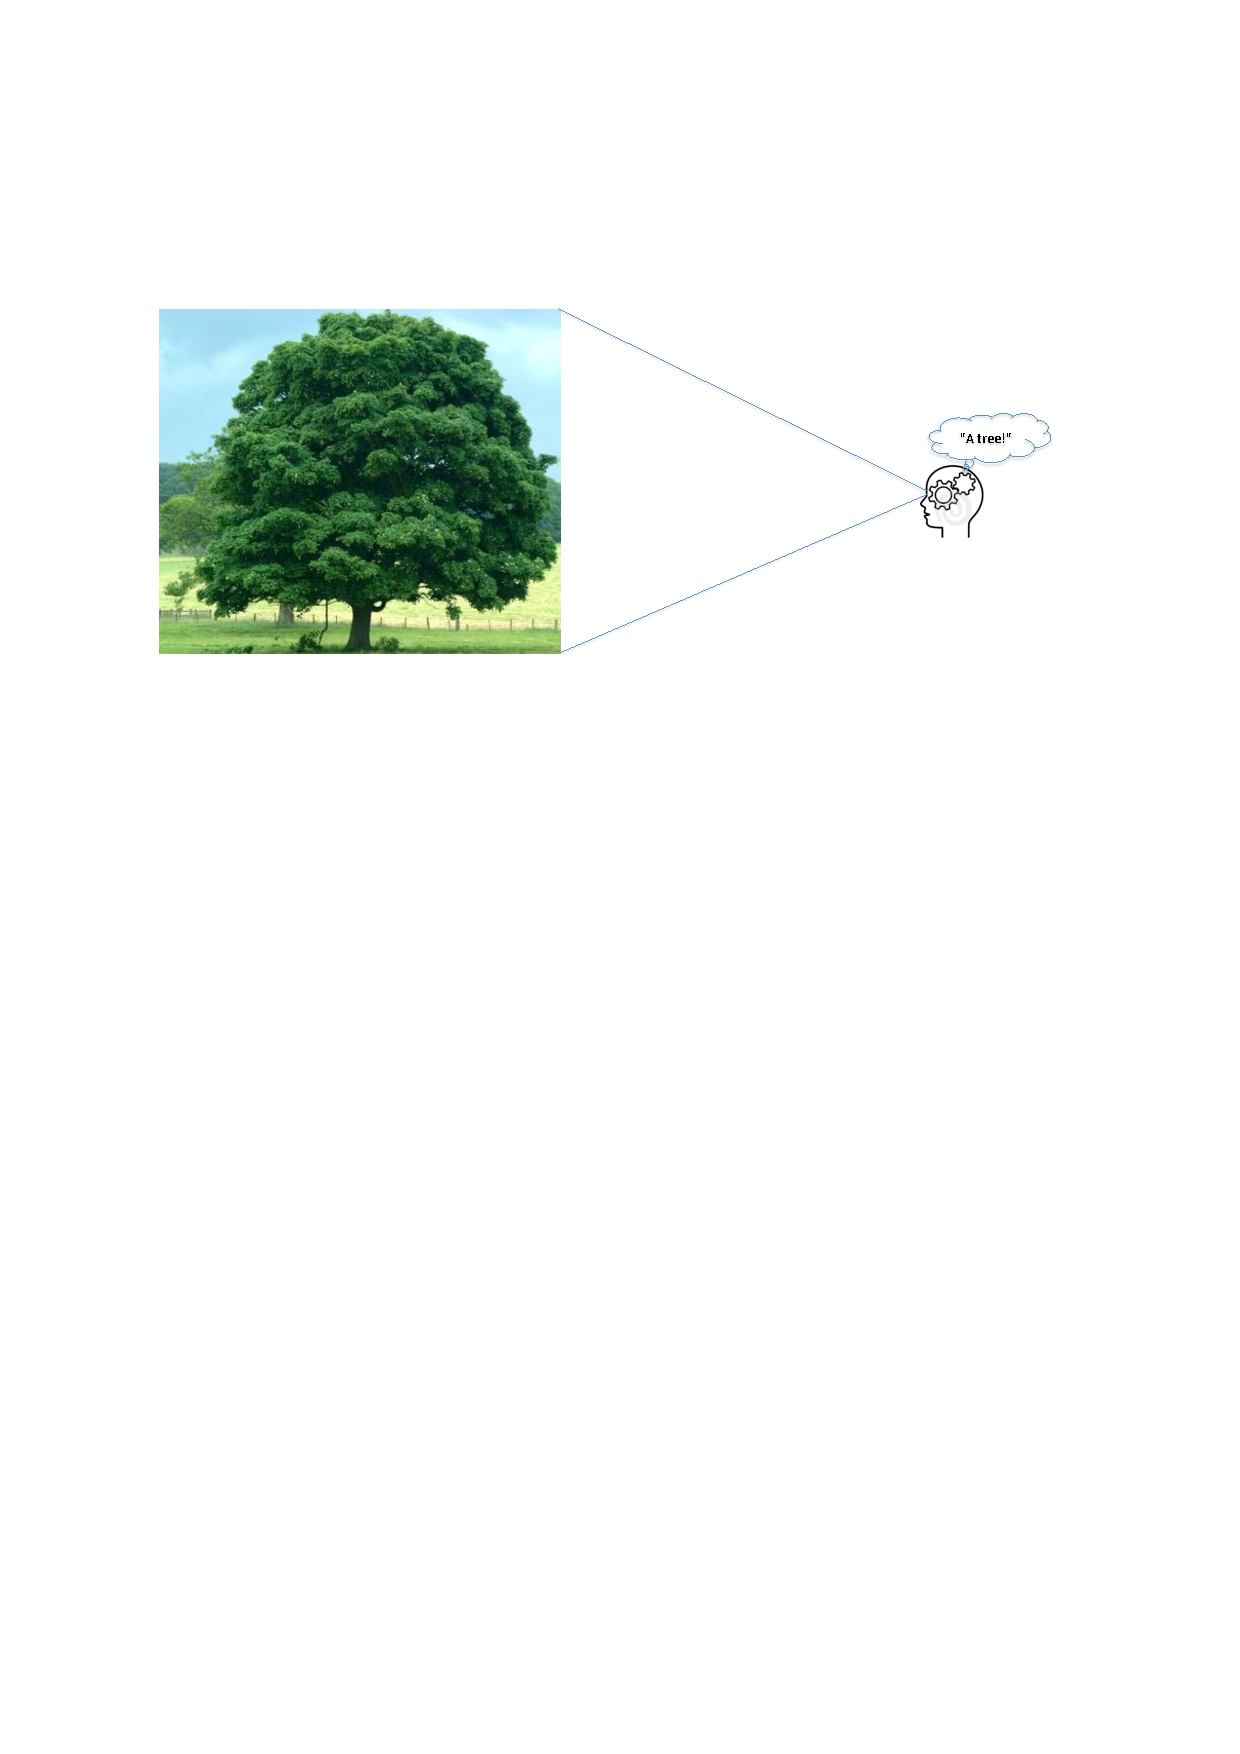
\includegraphics[width=4in]{seetree}

% }

% \frame{

% \frametitle{Seeing a tree}

% \only<1>{\textit{A Fregean view}

% 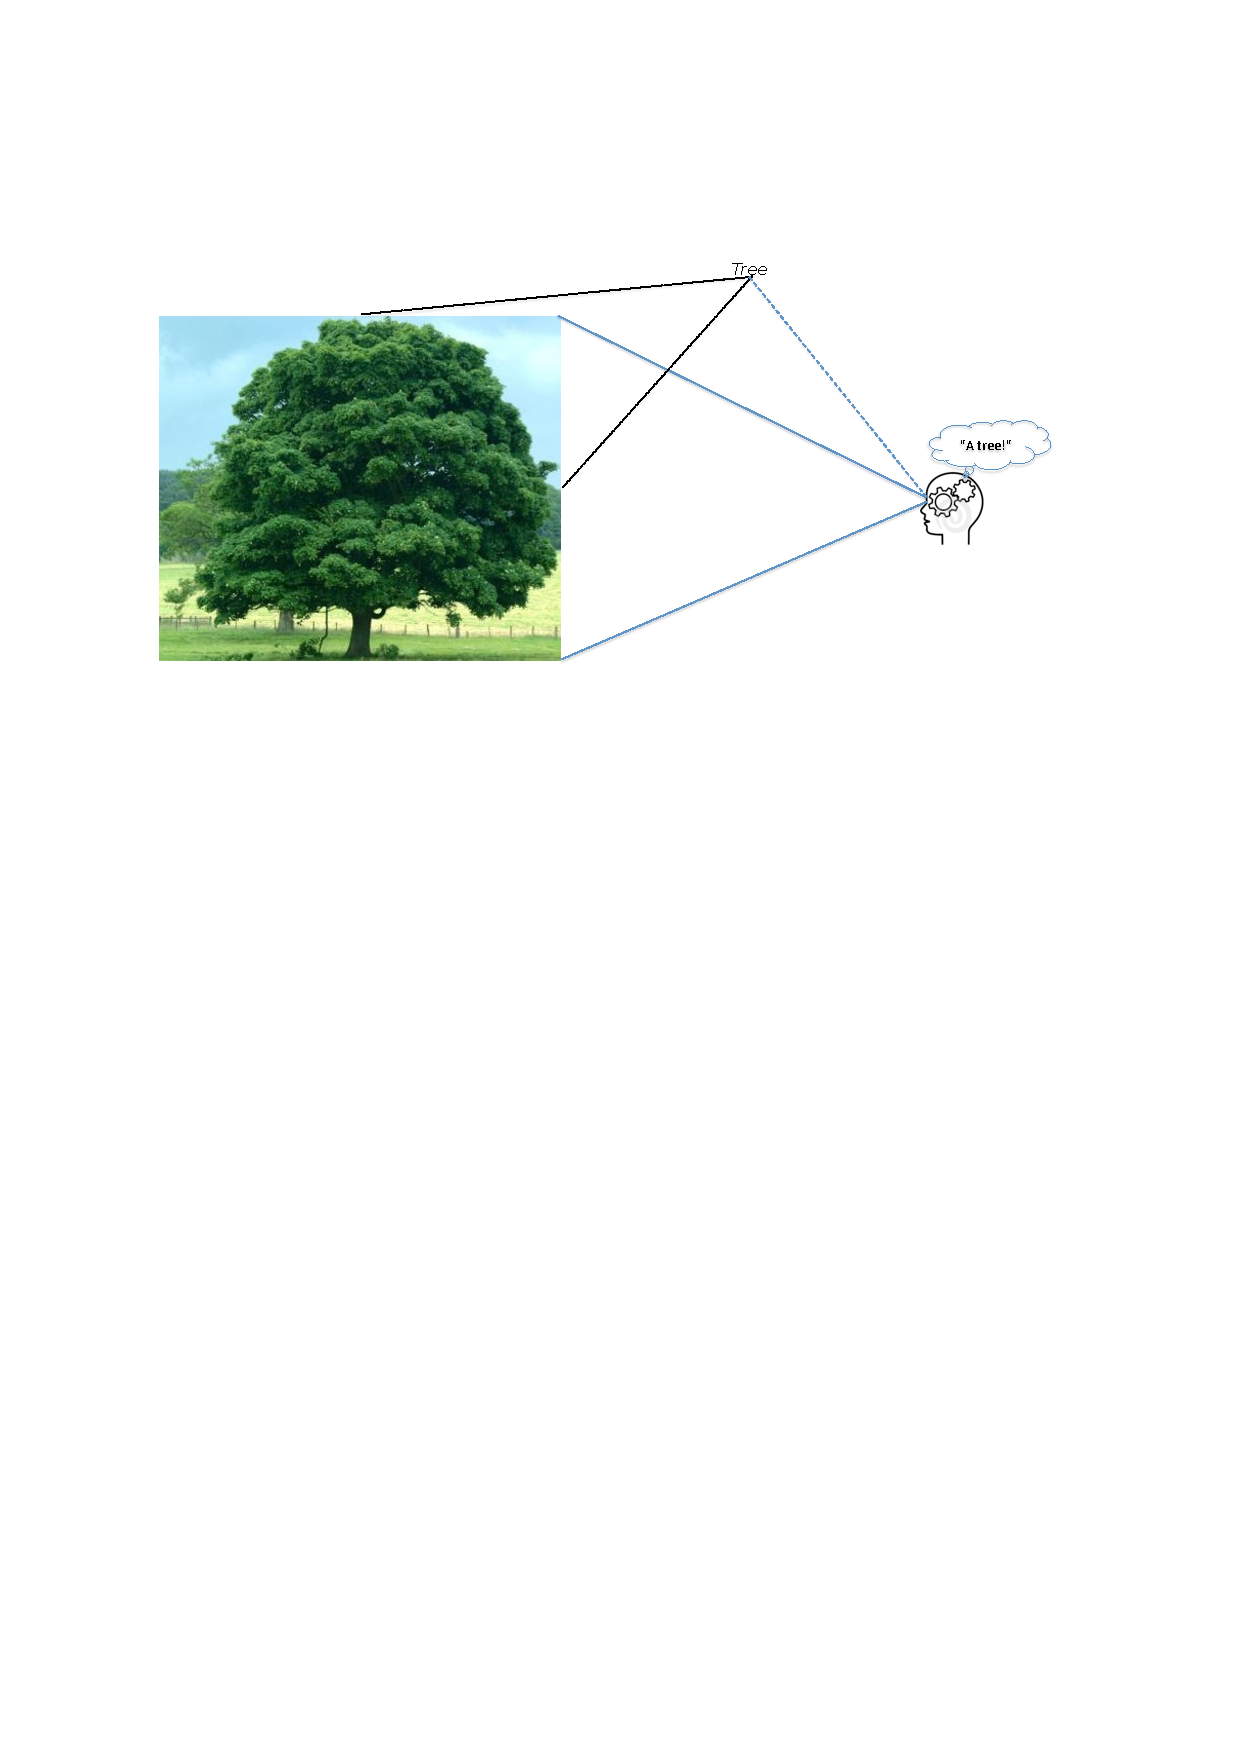
\includegraphics[width=4in]{seetreeFregean}}

% \only<2>{\textit{A mentalist view}

% \bigskip

% 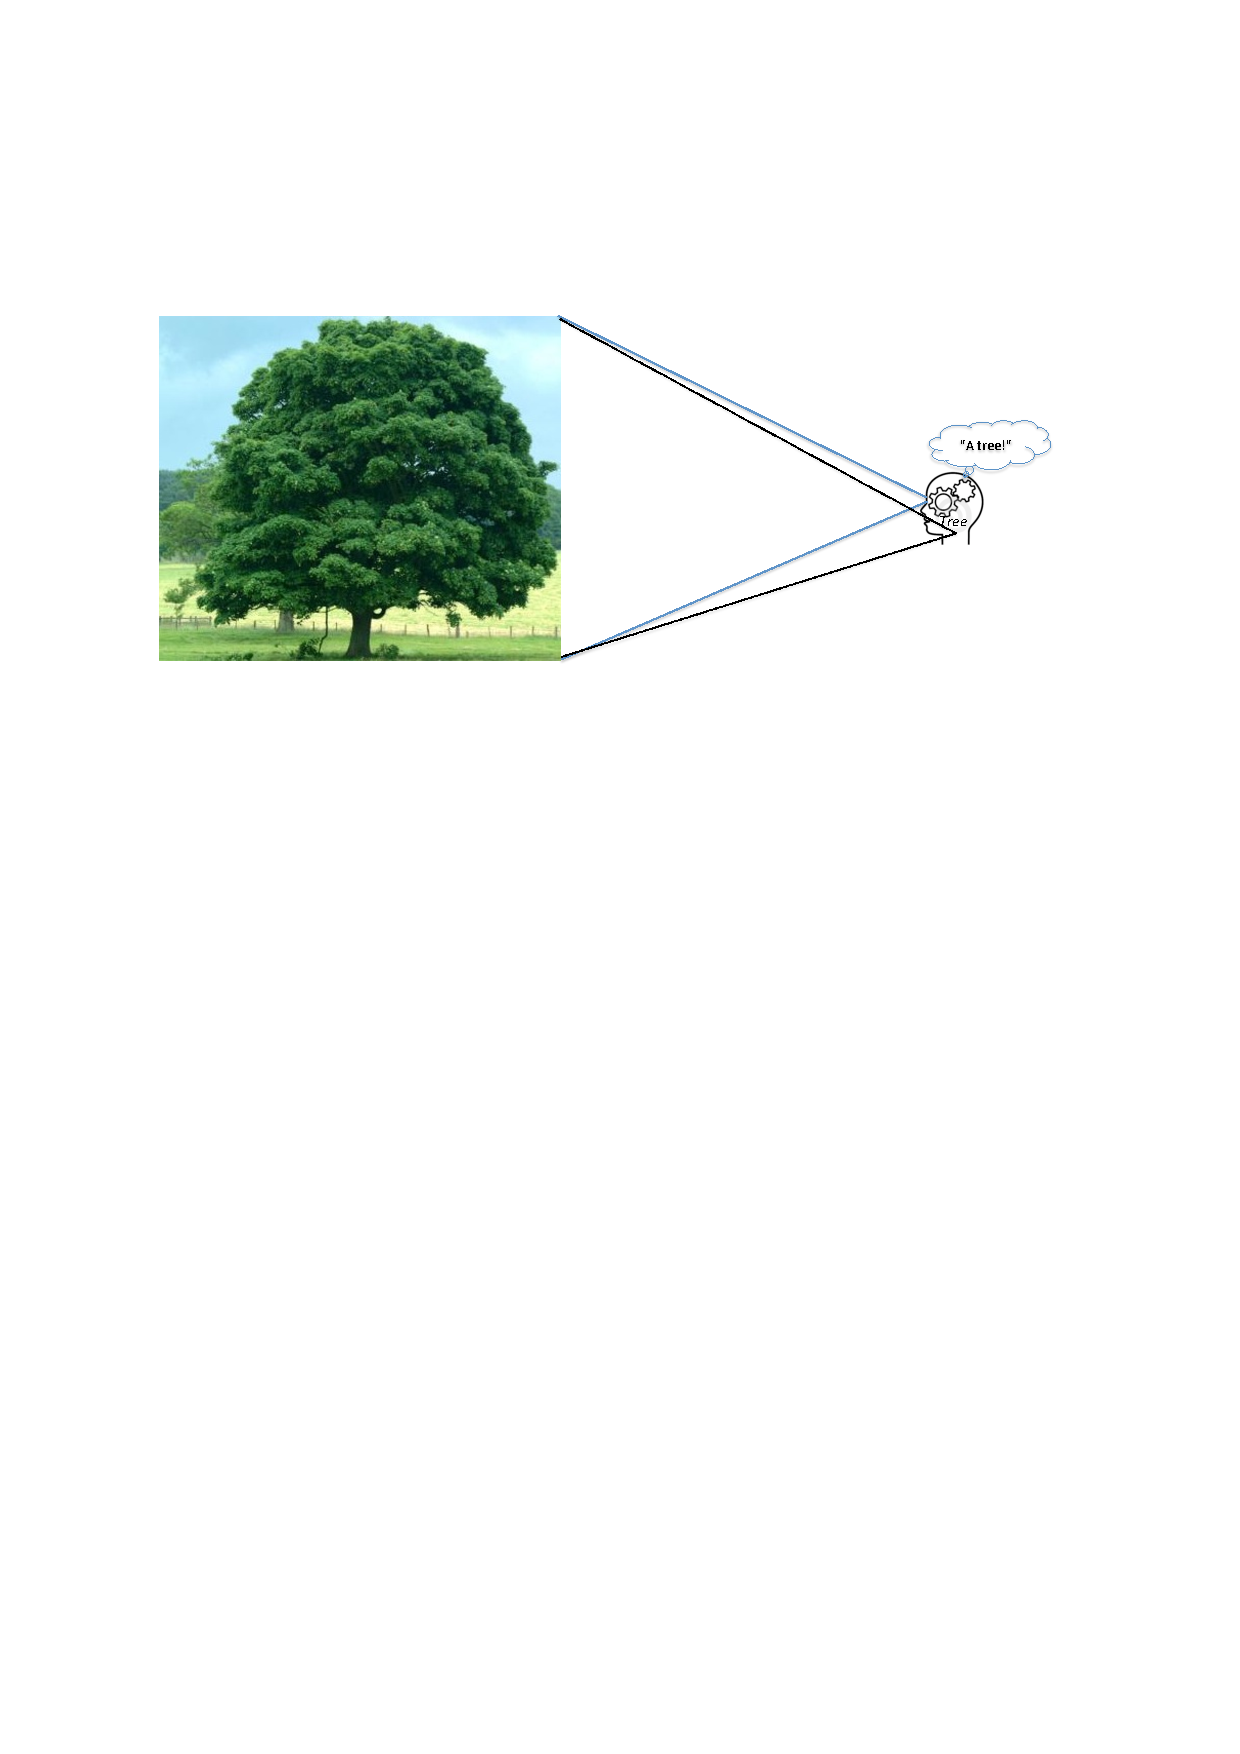
\includegraphics[width=4in]{seetreementalist}}

% }

\frame{

\frametitle{Seeing a tree (a simulation view)}

\begin{overprint}

\only<1>{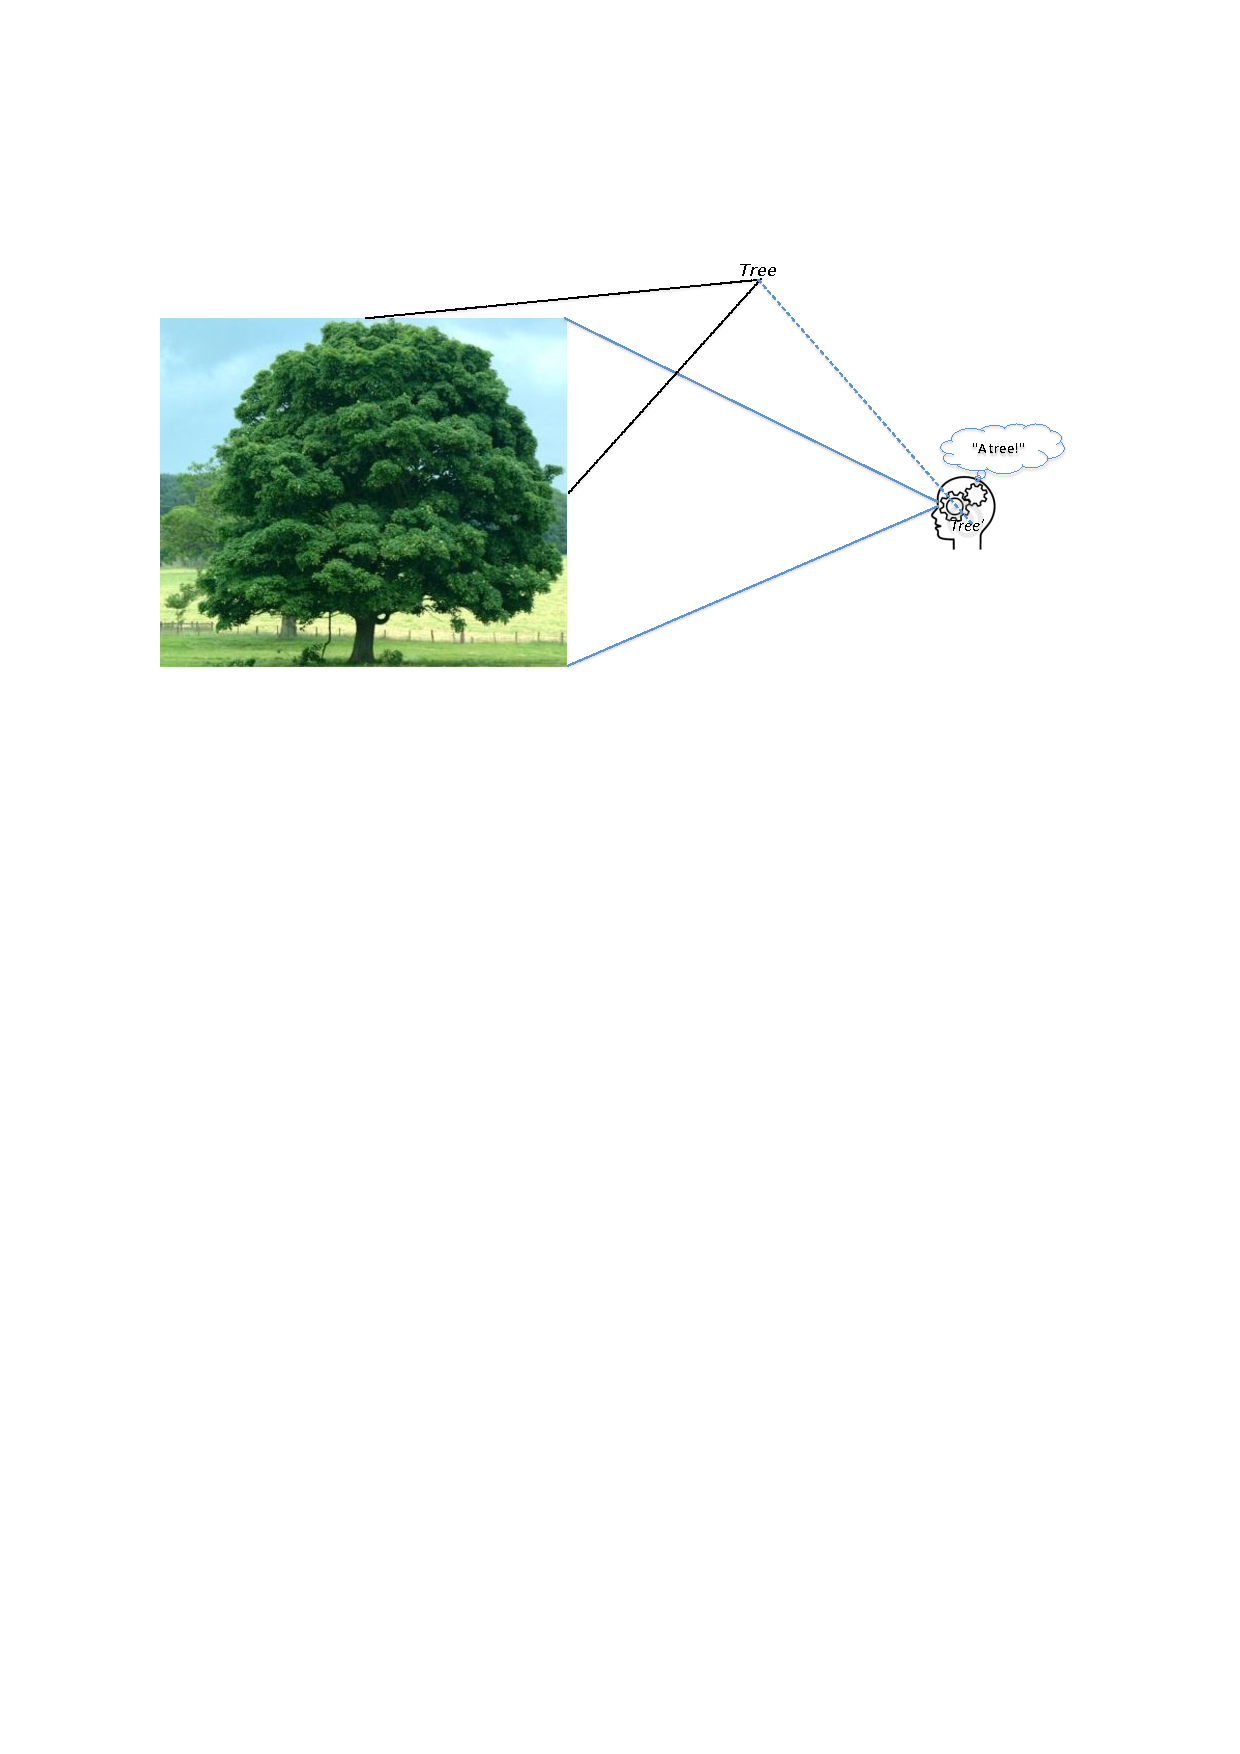
\includegraphics[width=3.4in]{seetreesimulation1}}
\only<2>{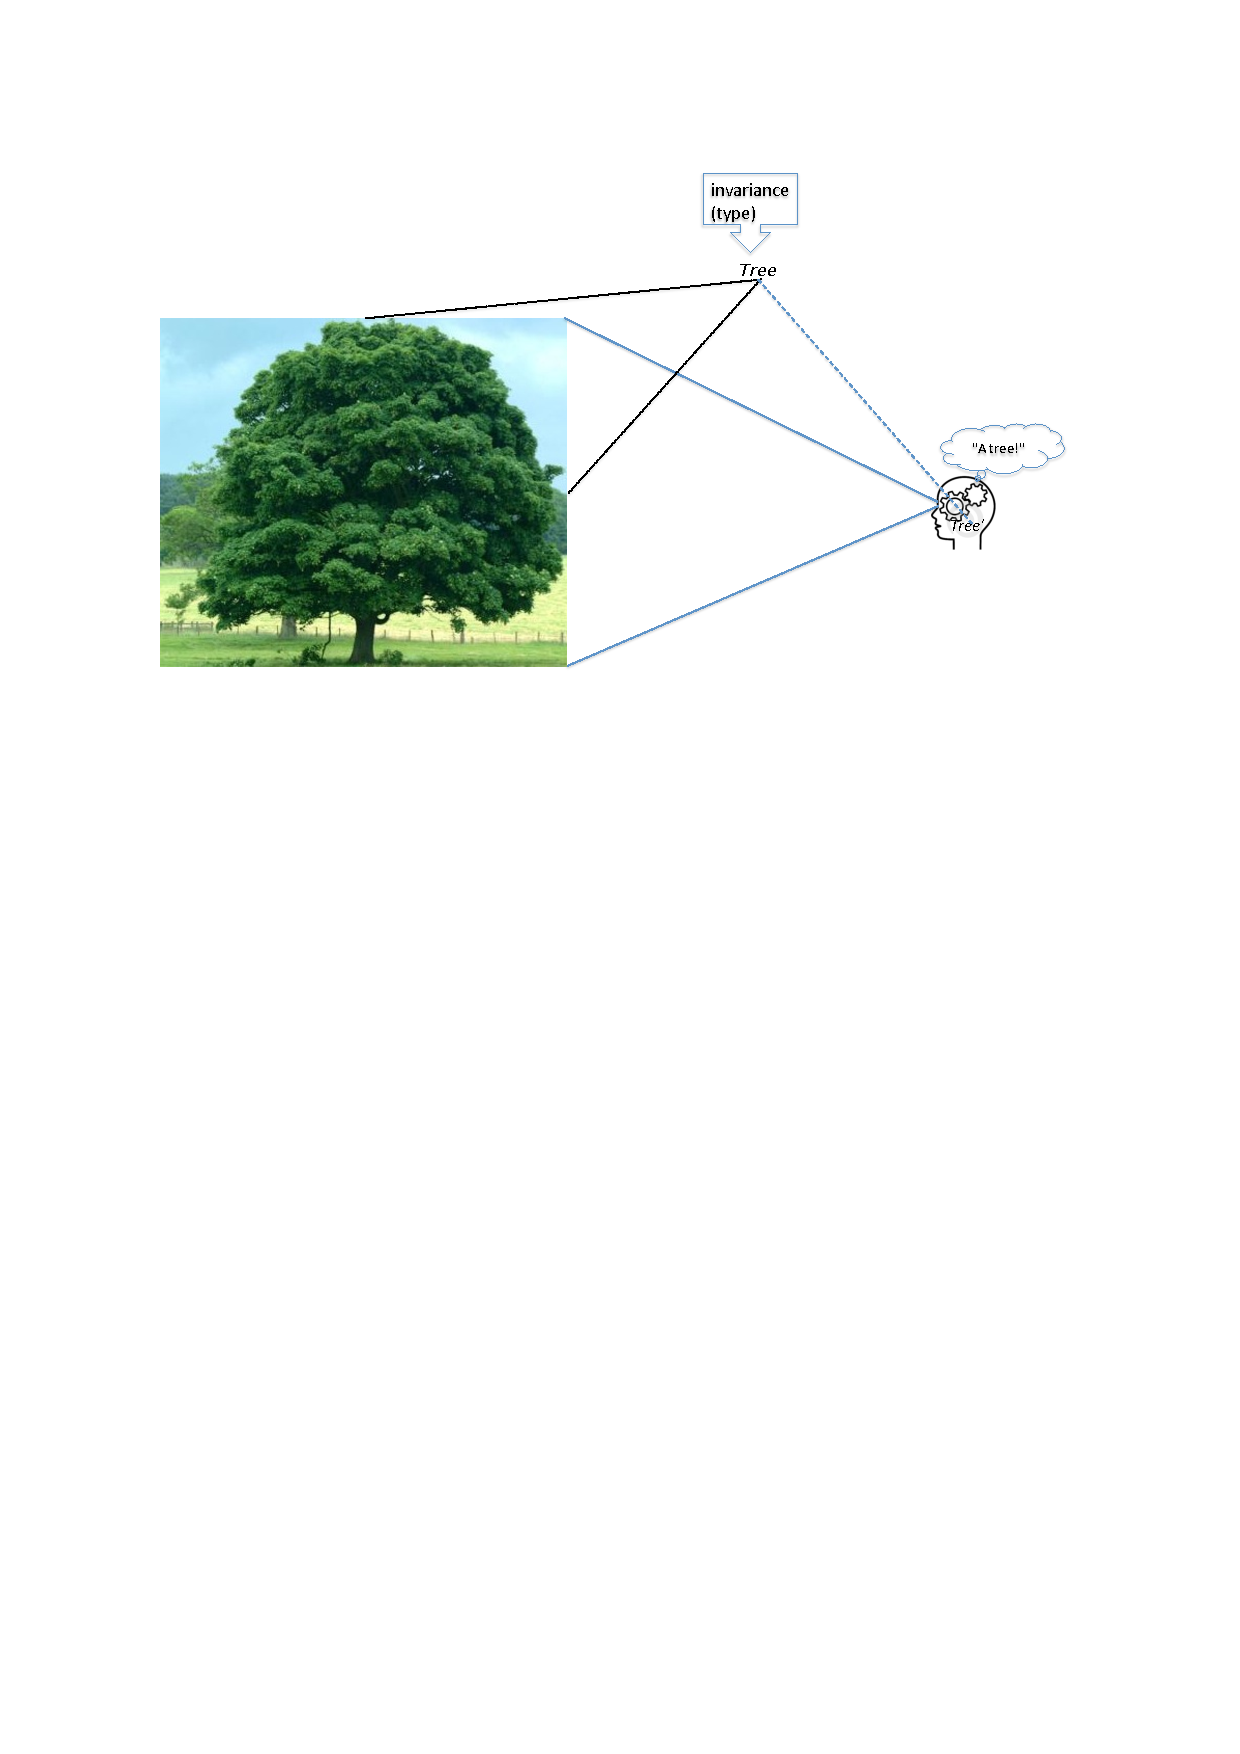
\includegraphics[width=3.4in]{seetreesimulation2}}
\only<3>{\vspace*{-.5em}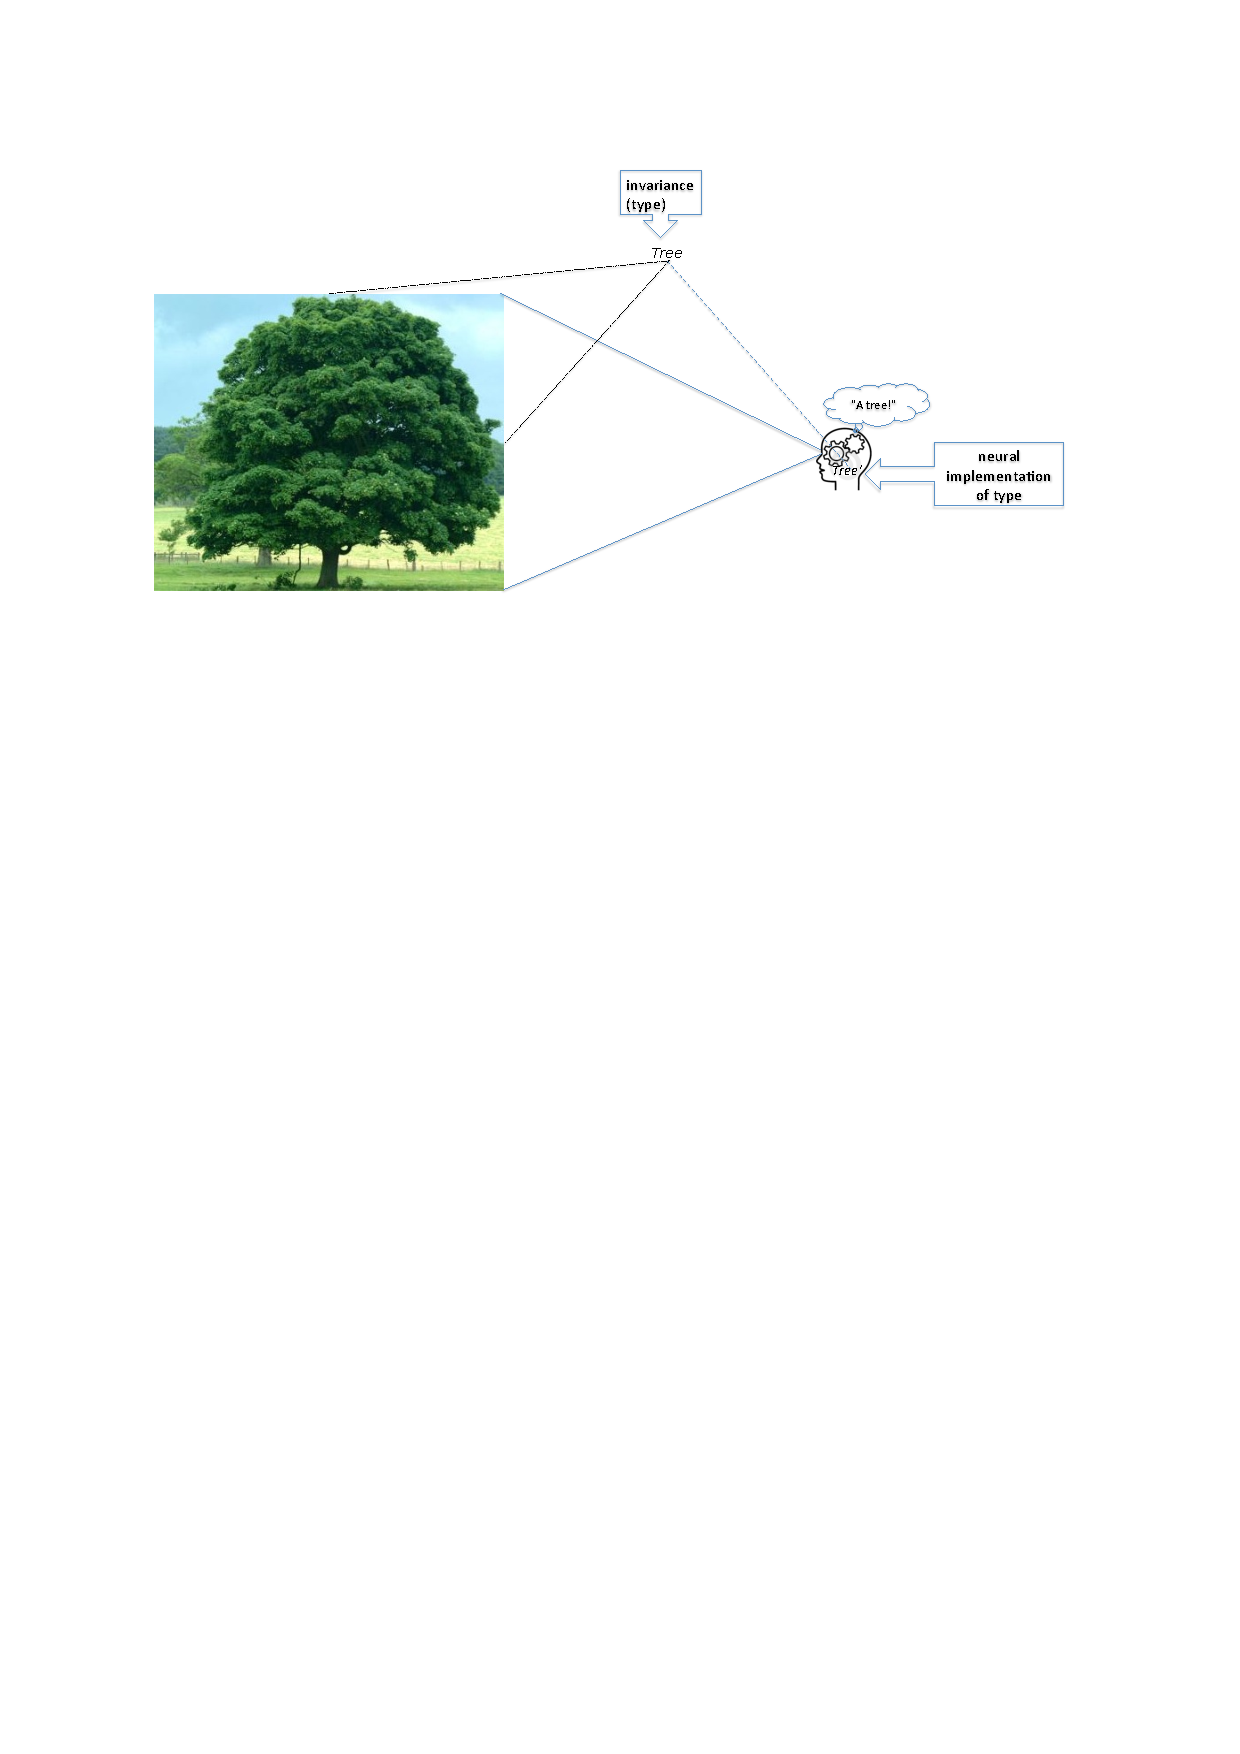
\includegraphics[width=3.96in]{seetreesimulation3}}
\only<4-5>{\vspace*{-.5em}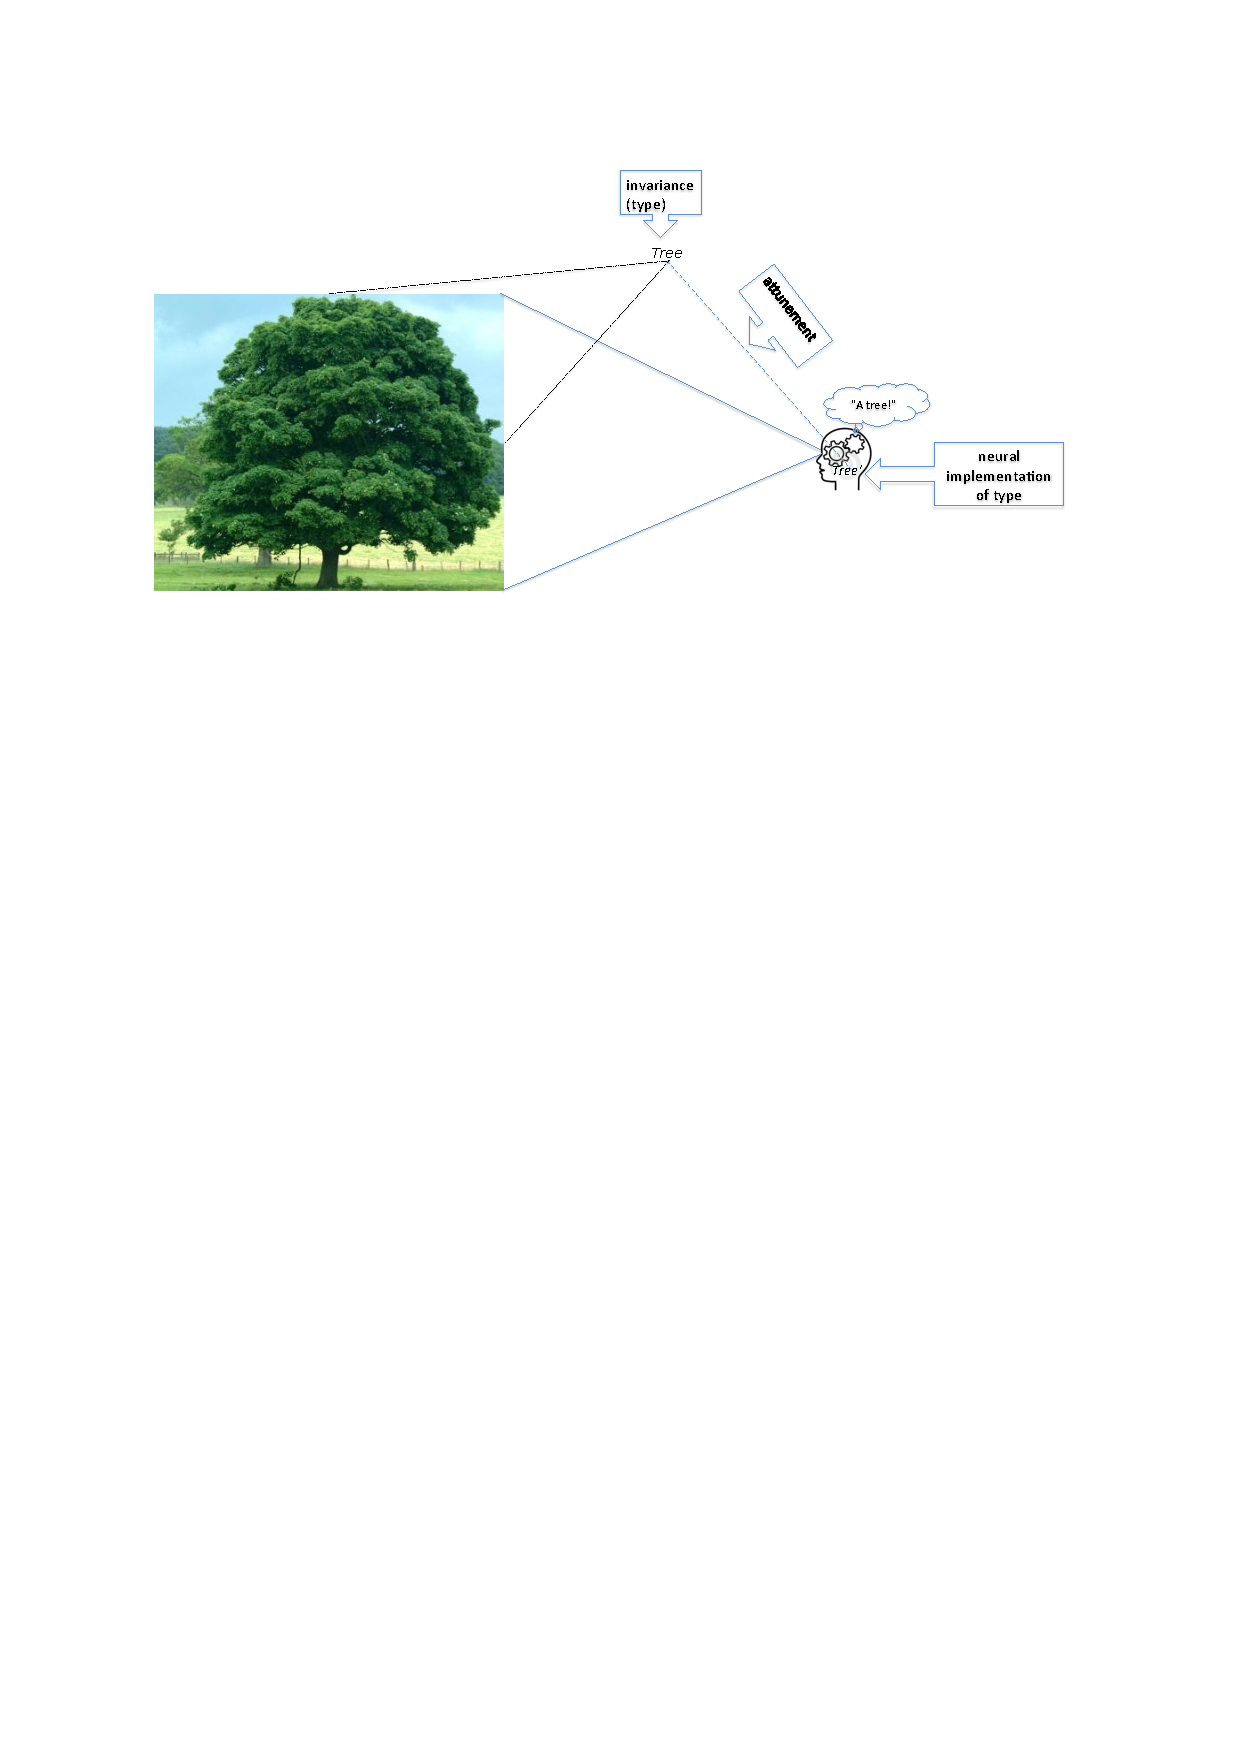
\includegraphics[width=3.96in]{seetreesimulation4}}

\end{overprint}

\only<5>{\cite{Gibson1986,BarwisePerry1983}}

}

\frame{

\frametitle{Judgement}


\begin{itemize} 
 
\item (An agent judges that) object $a$ is of type $T$. 
 
\item $a:T$ 

 
\end{itemize} 

}

\section{TTR:  Type theory with records}

\frame{

\frametitle{TTR: Type theory with records}

\begin{itemize} 
 
\item The most recent published reference for the details is \cite{Cooper2012} 
 
\item Also \cite{Cooper2005} for an earlier detailed treatment

\item \cite{Cooper2005a} for relation to various semantic theories

\item
  \url{https://sites.google.com/site/typetheorywithrecords/drafts/ch1-draft111114.pdf}
  for some current work in progress we will discuss here
 
\end{itemize} 

} 

\frame{

\frametitle{Rich type theory}

\begin{itemize} 
 
\item \textit{traditional type theories}
  \citep[e.g.][]{Montague1973,Montague1974} provide types for basic
  ontological classes (e.g., for Montague, entities, truth values,
  time points, possible worlds
  and total functions between these objects) 
 
\pause \item \textit{rich type theories} \citep[e.g.][]{Martin-Loef1984}
  provide a more general types, e.g. in our type theory, categories of
  objects such as \textit{Tree}, types of situations such as
  \textit{Hugging of a dog by a boy} 

\pause \item two fundamental questions when characterizing a type theory:

\begin{itemize} 
 
\item what types are there? 
 
\item for any type, what are the objects of that type? 
 
\end{itemize} 
  
 
\end{itemize} 
  

}

\frame{

\frametitle{Basic types}

\begin{itemize} 
 
\item basic types (as opposed to complex ones) are types which are not
  constructed from smaller parts  
 
\pause \item a system of basic types contains a set of such types,
  \textbf{Type}

\pause \item examples:  \textit{Ind} (``individual''), \textit{Time} (``time
  point'')

\pause \item a system of basic types also contains a function, $A$, which
  assigns a set of objects to each of the types in \textbf{Type}

\pause \item $a:T$ iff $a\in A(T)$

\end{itemize}

}

\frame{

\frametitle{Intensionality}

\begin{itemize}

\item Important: types are mathematical objects in their own right,
  they are not just sets of objects.

\pause \item Consequence: you can have two distinct types which have the same set of
  objects associated with them, i.e. $A(T_1)=A(T_2)$, $a:T_1$ just in
  case $a:T_2$.  The types are \textit{intensional}.
 
\end{itemize}

} 
     

% \frame{

% \frametitle{System of basic types}

% A {\it system of basic types\/} is a pair:
% \begin{display}
% {\bf TYPE$_B$} = $\langle${\bf Type}, $A$$\rangle$
% \end{display}
% where:
% \begin{enumerate} 
 
% \item \textbf{Type} is a non-empty set 
 
% \item $A$ is a function whose domain is \textbf{Type}

% \item for any $T\in\textbf{Type}$, $A(T)$ is a set disjoint from
%   \textbf{Type}

% \item for any $T\in\textbf{Type}$, $a:_{\mathbf{TYPE_B}}T$ iff $a\in A(T)$
 
% \end{enumerate}



% }

\frame{

\frametitle{$a:T_1$}

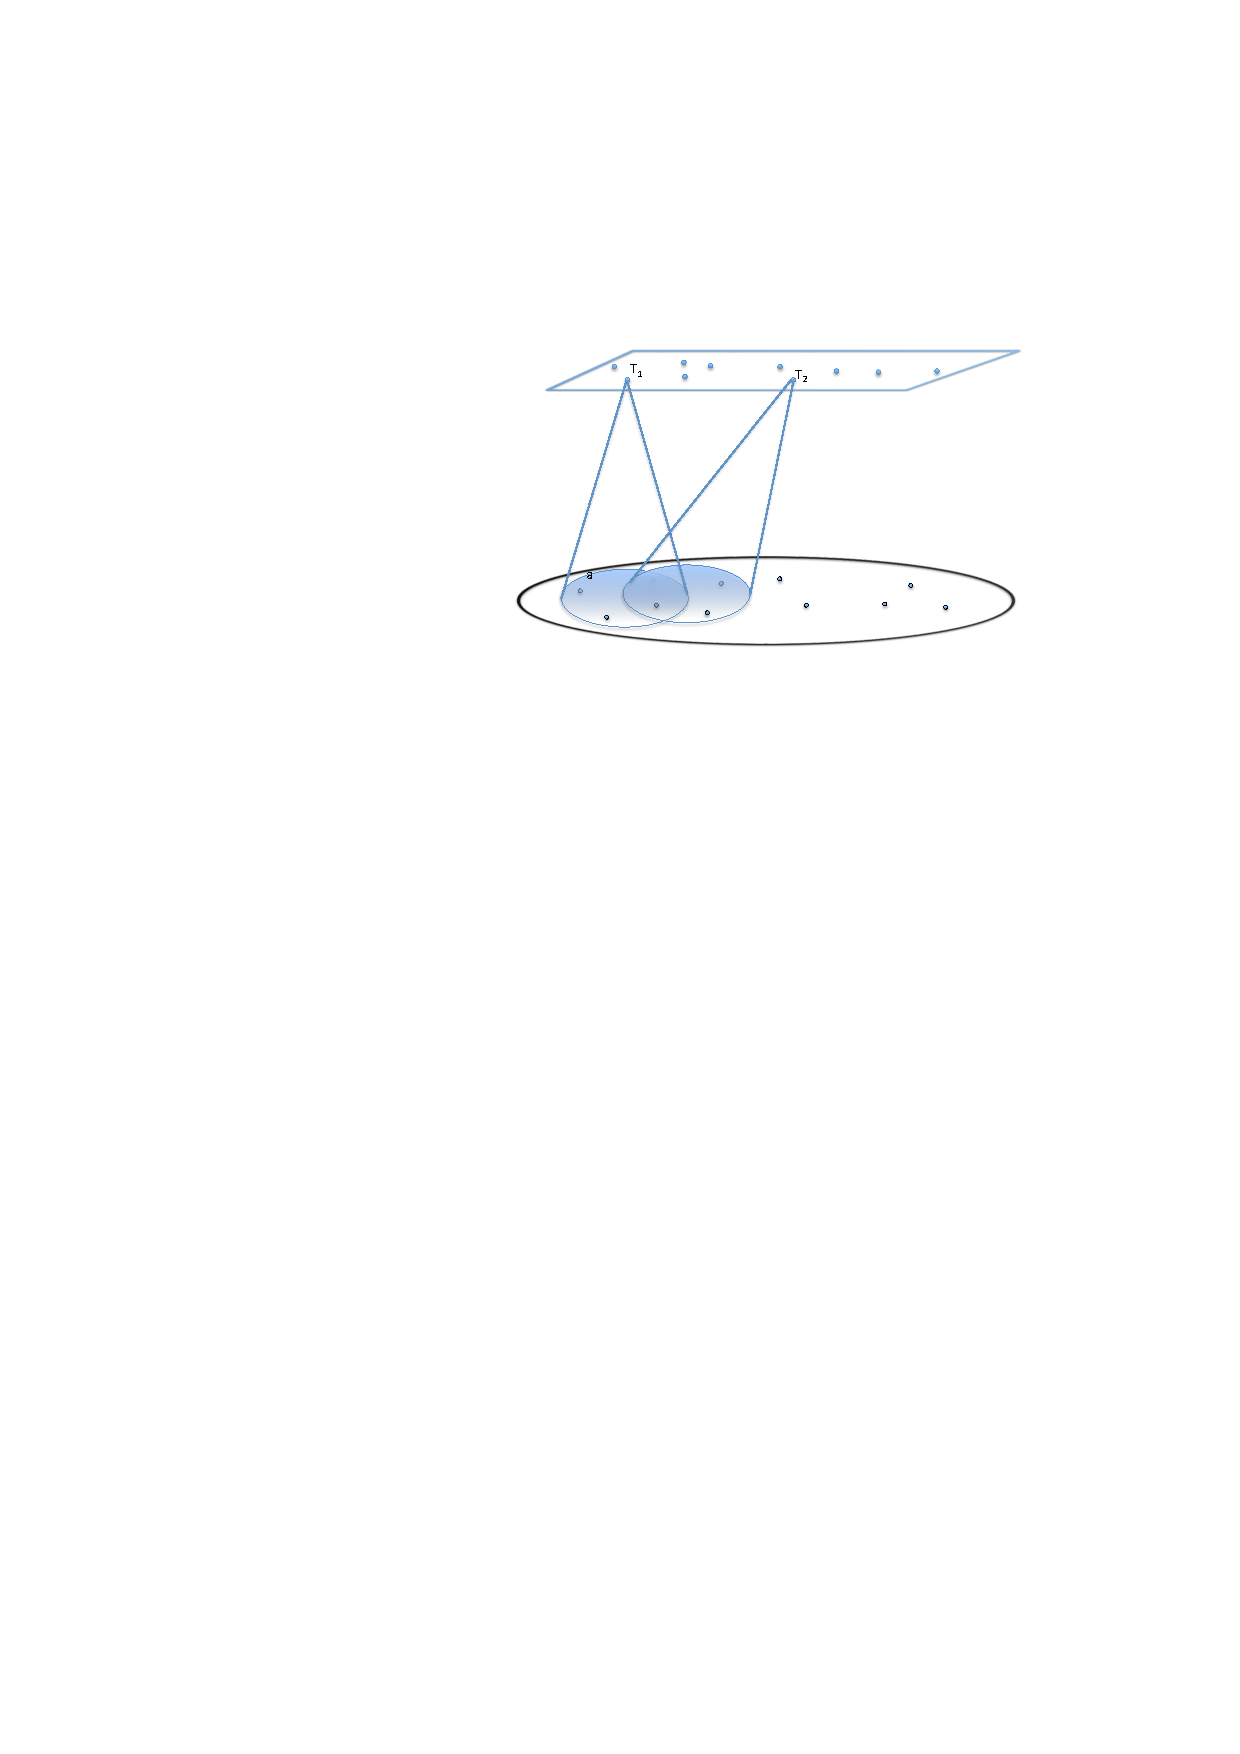
\includegraphics[width=4in]{basic}

}

\frame{

\frametitle{Types may be structured mathematical objects}

\begin{itemize} 
 
\item types may be constructed from other mathematical objects 
 
\item that is, they are \textit{complex} types (\textit{non-basic}
  types)

\pause \item one kind of complex type is \textit{ptype}, types which are
  constructed from predicates and objects used as arguments to the
  predicate

\pause \item another kind of complex type is \textit{record type}, types
  which consist of a collection of types indexed by labels
 
\end{itemize} 

} 

\frame{

\frametitle{Why is structure important?}

\begin{itemize} 
 
\pause \item increases intensionality (e.g. same ``content'', different structure)
 
\pause \item allows us to find parts within a whole (e.g. in clarification)

\pause \item allows us to modify by adding or removing a part (e.g. in
  learning new meanings or coordinating meaning with your dialogue partner)
 
\end{itemize} 

}   


\frame{

\frametitle{Seeing a hugging event}

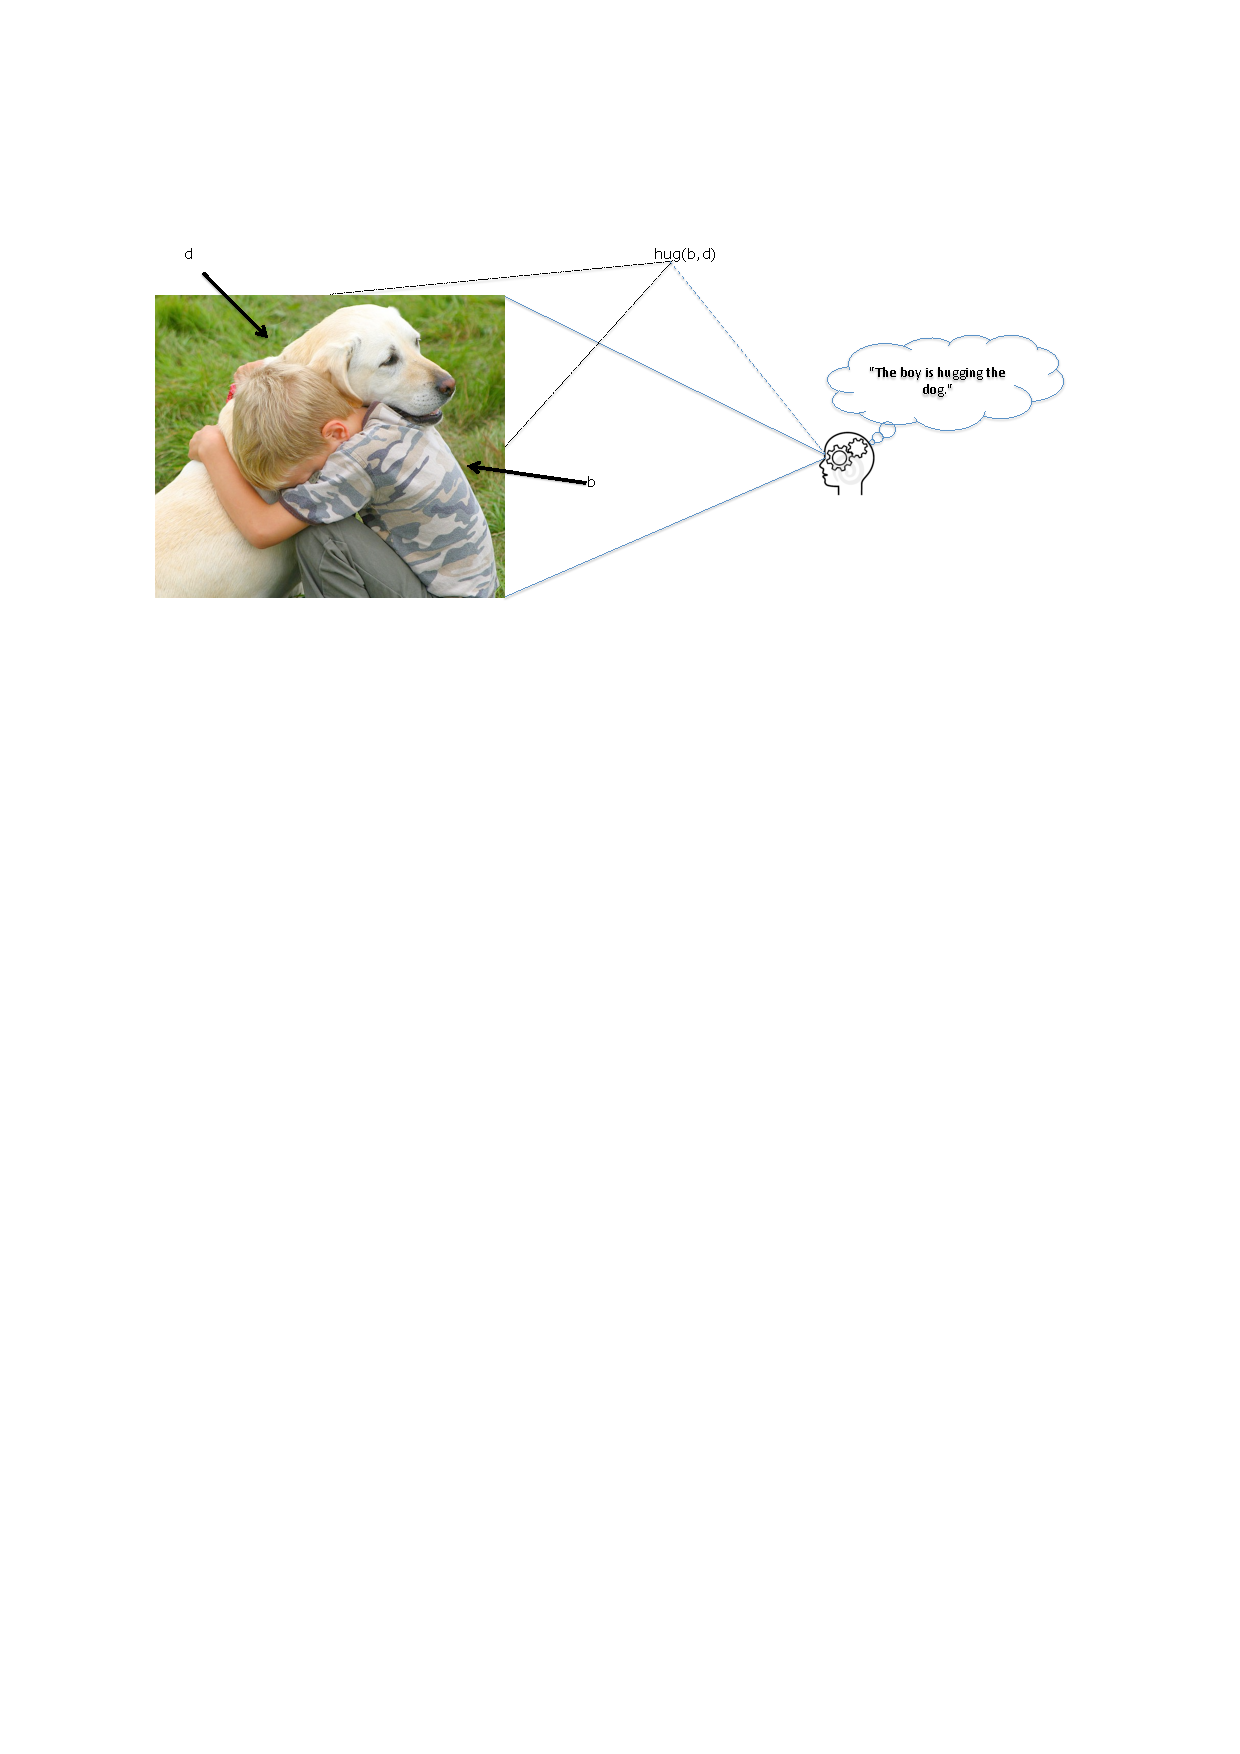
\includegraphics[width=4in]{seehug}

}

\frame{

\frametitle{Predicates}

\begin{itemize} 
 
\item predicates such as `run', `hug' 
 
\pause \item predicates come along with an \textit{arity} which tells you
  what kind of \textit{arguments} the predicates have:

\begin{itemize} 
 
\item Arity(run) = $\langle$\textit{Ind}$\rangle$ 
 
\item Arity(hug) = $\langle$\textit{Ind}, \textit{Ind}$\rangle$ 
 
\end{itemize} 

\pause \item We might also want to include time intervals and locations as
  part of the arities of these predicates
 
\end{itemize} 

}

  

% \frame{

% \frametitle{Predicate signatures}

% A \textit{predicate signature} 
% is a triple
% \begin{display}
% $\langle$\textbf{Pred}, \textbf{ArgIndices}, \textit{Arity}$\rangle$
% \end{display}
% where:
% \begin{enumerate} 
 
% \item \textbf{Pred} is a set (of predicates)

% \item \textbf{ArgIndices} is a set (of indices for predicate
%   arguments, normally types)
 
% \item \textit{Arity} is a function with domain \textbf{Pred} and range
%   included in the set of finite sequences of members of \textbf{ArgIndices}. 
 
% \end{enumerate}

% }

% \frame{

% \frametitle{Polymorphic predicate signatures}

% A \textit{polymorphic predicate signature} 
% is a pair 
% \begin{display}
% $\langle$\textbf{Pred}, \textbf{ArgIndices}, \textit{Arity}$\rangle$
% \end{display}
% where:
% \begin{enumerate} 
 
% \item \textbf{Pred} is a set (of predicates)

% \item \textbf{ArgIndices} is a set (of indices for predicate
%   arguments, normally types)
 
% \item \textit{Arity} is a function with domain \textbf{Pred} and range
%   included in the powerset of the set of finite sequences of members
%   of \textbf{ArgIndices}. 
 
% \end{enumerate}

% }

\frame{

\frametitle{Ptypes}

\begin{itemize} 
 
\item ptypes are constructed from predicates and arguments
  corresponding to their arities 
 
\pause \item examples:  run($d$), hug($b$,$d$) (where $b$,$d$:\textit{Ind})

\pause \item ptypes are types of situations (events)

\pause \item a system of complex types will contain a set of ptypes, \textbf{PType}, in
  addition to basic types

\pause \item \textbf{PType} will be based on a set of predicates with their
  arities

\pause \item \textbf{PType} will contain all the possible ptypes for a given
  predicate given what is assigned to the arity for the predicate
  elsewhere in the system

\pause \item a system of complex types will also contain a function, $F$,
  which assigns a set, possibly empty, (of situations) to each ptype.
 
\end{itemize} 

} 

\frame{

\frametitle{Models}

\begin{itemize} 
 
\item $A$ and $F$ together, that is, $\langle A,F\rangle$, is a \textit{model} 
 
\item a model consists of an assignment to the basic types and an
  assignment to the ptypes

\pause \item note that a model in this sense is \textit{part} of the type
  system (not an external interpretation of it)

\item this is an important difference between rich type theories and
  traditional model theory
 
\end{itemize} 

}   

% \frame[plain]{

% \frametitle{System of complex types}

% A {\it system of complex types\/} is a quadruple:
% \begin{display}
% {\bf TYPE$_C$} = $\langle${\bf Type}, {\bf BType},
% $\langle$\textbf{PType}, {\bf Pred}, \textbf{ArgIndices}, {\it Arity\/}$\rangle$, $\langle A,F\rangle$$\rangle$
% \end{display}
% where:  
% \begin{enumerate} 
 
% \item $\langle$\textbf{BType}, $A$$\rangle$ is a system of basic types 
 
% \item \textbf{BType}$\subseteq$\textbf{Type}

% \item for any $T\in\textbf{Type}$, if $a:_{\langle\mathbf{BType},
%     A\rangle}T$ then $a:_{\mathbf{TYPE_C}}T$

% \item \label{cl:predtypes}$\langle${\bf Pred}, \textbf{ArgIndices},
%   {\it Arity\/}$\rangle$ is a (polymorphic) predicate
%   signature

% \item \sloppy If $P\in\textbf{Pred}$, $T_1\in \mathbf{Type},\ldots,T_n\in
%   \mathbf{Type}$, \textit{Arity}($P$)=$\langle
%   T_1,\ldots,T_n\rangle$  ($\langle
%   T_1,\ldots,T_n\rangle$$\in$\textit{Arity}($P$)) and $a_1:_{\mathbf{TYPE_C}}T_1,\ldots,a_n:_{\mathbf{TYPE_C}}T_n$ then
%   $P(a_1,\ldots a_n)\in\textbf{PType}$

% \item \textbf{PType}$\subseteq$\textbf{Type}

% \item for any $T\in\textbf{PType}$, $F(T)$ is a set disjoint from \textbf{Type}

% \item for any $T\in\textbf{PType}$, $a:_{\mathbf{TYPE_C}}T$ iff $a\in F(T)$
 
% \end{enumerate}
% }

\frame{

\frametitle{Are ptypes the only types of situations?}

\begin{itemize} 
 
\item suppose $b$ is Bill, a boy and $d$ is Dinah, a dog 
 
\item we have allowed ourselves the ptype hug($b$,$d$), the type of
  situation where Bill hugs Dinah

\item but we have not allowed ourselves the type of ``boy hugs dog''
  situations corresponding to \textit{a boy hugs a dog}

\item there are a number of ways to construct such types in rich type
  theories -- we use \textit{record types}
 
\end{itemize}   


}

\frame{

\frametitle{A boy hugs a dog}

Record type -- ``a collection of labelled types''

\only<2>{\ldots not quite because of dependencies}

\begin{center}

\record{\tfield{x}{\textit{Ind}} \\
        \tfield{c$_{\mathrm{boy}}$}{boy(x)} \\
        \tfield{y}{\textit{Ind}} \\
        \tfield{c$_{\mathrm{dog}}$}{dog(y)} \\
              \tfield{e}{hug(x,y)}} 
\end{center}
}



\frame{

\frametitle{The official notation}

\begin{center}

\record{\tfield{x}{\textit{Ind}} \\
        \tfield{c$_{\mathrm{boy}}$}{$\langle\lambda
          v:\mathit{Ind}$(boy($v$)),$\langle$x$\rangle\rangle$,} \\
        \tfield{y}{\textit{Ind}} \\
        \tfield{c$_{\mathrm{dog}}$}{$\langle\lambda
          v:\mathit{Ind}$(dog($v$)),$\langle$y$\rangle\rangle$} \\
              \tfield{e}{$\langle\lambda
                v_1:\mathit{Ind}(\lambda
                v_2:\mathit{Ind}$(hug($v_1$,$v_2$))),\\
&&\hspace*{2em}$\langle$x,y$\rangle\rangle$}}

\end{center}

}

\frame{

\frametitle{A record of type \textit{a boy hugs a dog}}

\begin{center}

\record{\field{x}{$a$} \\
        \field{c$_{\mathrm{boy}}$}{$s_1$} \\
        \field{y}{$b$} \\
        \field{c$_{\mathrm{dog}}$}{$s_2$} \\
        \field{e}{$s_3$}}
\end{center}

\begin{center}
\begin{tabular}{ll}
where: & $a$ : \textit{Ind} \\
       & $s_1$ : boy($a$) \\
       & $b$ : \textit{Ind} \\
       & $s_2$ : dog($b$) \\
       & $s_3$ : hug($a$,$b$)
\end{tabular}
\end{center}


}

\frame{

\frametitle{Two important facts about records}

\begin{itemize} 
 
\item You can construct a record of a given type just in case there
  are objects of the types required by its fields -- i.e. the
  labelling is arbitrary  
 
\pause \item A record of a given type may contain more fields than required
  by the type -- this record also belongs to a subtype of the type
  where the extra fields are added
 
\end{itemize} 


}

\frame{

\frametitle{Why are record types interesting for linguists?}

\begin{itemize} 
 
\item they allow us to model discourse representation structures 
 
\pause \item they allow us to model feature structures 

\pause \item they allow us to model dialogue game boards (information
states)

\pause \item they allow us to model frames (as in frame semantics and FrameNet)
 
\end{itemize} 


}  


% \frame{

% \frametitle{Function types}

% \textbf{TYPE}$_C$ \textit{has function types} if
% \begin{enumerate} 
 
% \item for any $T_1,T_2 \in \mathbf{Type}$, $(T_1\rightarrow T_2) \in \mathbf{Type}$ 
 
% \item for any $T_1,T_2 \in \mathbf{Type}$, $f:_{\mathbf{TYPE_C}}(T_1\rightarrow T_2)$ iff
%   $f$ is a function whose domain is $\{a\mid
%   a:_{\mathbf{TYPE_C}}T_1\}$ and whose range is included in $\{a\mid a:_{\mathbf{TYPE_C}}T_2\}$ 
 
% \end{enumerate}

% }

% \frame{

% \frametitle{Records}

% \begin{itemize}

% \item A {\it record\/} is a finite set of ordered pairs (called {\it fields\/})
% which is the graph of a function.  If $r$ is a record and $\langle\ell,v\rangle$
% is a field in $r$ we call $\ell$ a {\it label\/} and $v$ a {\it value\/} in $r$
% and we use $r.\ell$ to denote $v$.  $r.\ell$ is called a \textit{path}
% in $r$.  If $\pi$ is a path in $r$ whose denotation is itself a record
% with a label $\ell$, then $\pi.\ell$ is also a path in $r$.

% \pause \item A record $r$ is \textit{well-typed} with respect to a system of types
% \textbf{TYPE} with set of types \textbf{Type} and a set of labels $L$
% iff for each field $\langle\ell,a\rangle\in r$, $\ell\in L$ and
% $a:_\mathbf{TYPE}T$ for some $T\in\mathbf{Type}$.

% \end{itemize}

% }

% \frame[allowframebreaks]{

% \frametitle{Record types}

% A system of complex types \textbf{TYPE}$_C$ = $\langle${\bf Type}, {\bf BType},
% $\langle$\textbf{PType}, {\bf Pred}, \textbf{ArgIndices}, {\it
%   Arity\/}$\rangle$, $\langle A,F\rangle$$\rangle$ \textit{has record
%   types based on $\langle L, \mathbf{RType}\rangle$}, where $L$ is a countably infinite set (of labels)
% and \textbf{RType} $\subseteq$ \textbf{Type}, 
% defined by:
% \begin{enumerate} 
 
% \item $\mathit{Rec}\in\mathbf{RType}$
 
% \item $r:_{\mathbf{Type}_C}\mathit{Rec}$ iff $r$ is a well-typed record with
%   respect to \textbf{TYPE$_C$} and $L$.

% \item if $\ell\in L$ and $T\in\mathbf{Type}$, then
%   $\{\langle\ell,T\rangle\}\in\mathbf{RType}$.

% \item $r:_{\mathbf{Type}_C}\{\langle\ell,T\rangle\}$ iff
%   $r:_{\mathbf{Type}_C}\mathit{Rec}$, $\langle\ell,a\rangle\in r$ and
%   $a:_{\mathbf{Type}_C}T$.

% \item if $R\in\mathbf{RType}$, $\ell\in L$, $\ell$ does not occur as a
%   label in $R$ (i.e. there is no field $\langle\ell',T'\rangle$ in $R$
%   such that $\ell'=\ell$), then
%   $R\cup\{\langle\ell,T\rangle\}\in\mathbf{RType}$.

% \item $r:_{\mathbf{Type}_C}R\cup\{\langle\ell,T\rangle\}$ iff
%   $r:_{\mathbf{Type}_C}R$, $\langle\ell,a\rangle\in r$ and
%   $a:_{\mathbf{Type}_C}T$.

% \item if $R$ is a member of {\bf RType}, $\ell\in L$  not occurring as a label in $R$, $T_1,\ldots,T_m\in\mathbf{Type}$, $R.\pi_1,\ldots,R.\pi_m$ are paths in
%     $R$  and
%     ${\cal F}$ is a function of type $((a_1:T_1)\rightarrow\ldots\rightarrow((a_m:T_m)\rightarrow\mathit{Type})\ldots)$, then $R \cup \{\langle\ell, \langle{\cal F}, \langle\pi_1,\ldots,\pi_m\rangle\rangle\rangle\}\in\mathbf{RType}$.
    
% \item $r :_{\mathbf{TYPE}_{\mathit{C}}}R\cup\{\langle\ell,
%   \langle{\cal F}, \langle\pi_1,\ldots,\pi_m\rangle\rangle\rangle\}$
%   iff $r :_{\mathbf{TYPE}_{\mathit{C}}} R$, $\langle\ell, a\rangle$ is a field
% in $r$,  $r.\pi_1:_{\mathbf{TYPE}_{\mathit{C}}}T_1,\ldots,r.\pi_m:_{\mathbf{TYPE}_{\mathit{C}}}T_m$ and  $a :_{\mathbf{TYPE}_{\mathit{C}}} {\cal F}(r.\pi_1,\ldots,r.\pi_m)$.  
 
 
% \end{enumerate} 

% }

% \frame{

% \frametitle{The type \textit{Type}}

% \begin{itemize} 
 
% \item The previous slide introduced the type \textit{Type} 
 
% \item $T:$\textit{Type} iff $T\in$\textbf{Type}

% \pause \item \textit{Type}$\in$\textbf{Type}

% \pause \item \textit{Type}:\textit{Type}

% \pause \item But suppose we allow some type to have the extension
%   $\{T\in\mathbf{Type}\mid T\not\ : T\}$ \ldots

% \pause \item This leads us to stratification.
 
% \end{itemize} 
% }



\section{Summary and bibliography}


\frame{

\frametitle{Summary}

\begin{itemize} 
 
\item Type theory as a formal theory related to perception 
 
\item A basic introduction to TTR: 

\begin{itemize} 
 
\item basic types (e.g. \textit{Ind}) 
 
\item ptypes (e.g. hug(Sam,Dinah)) 

\item models which supply objects of  basic types and ptypes

\item record types

\item mentioned some of their linguistic applications

 
\end{itemize} 
  
 
\end{itemize} 
  

}



\frame[allowframebreaks]

\frametitle{Bibliography}

%\bibliographystyle{acl}

\bibliographystyle{/Users/cooper/LaTeX/bib/mybib}
\bibliography{/Users/cooper/LaTeX/bib/bibliography}

}      


\end{document}

\frame{

\frametitle{Two kinds of partiality}
\begin{itemize} 
 
\item not all frames are perceived -- infer more 
 
\pause \item  individual frame type partially specified

\pause \item \record{\tfield{x}{\textit{Ind}} \\
                     \tfield{y}{\textit{Ind}} \\
                     \tfield{c$_1$}{bus-stop(y)} \\
                     \tfield{c$_2$}{near(x,y)} \\
                     \tfield{c$_3$}{wait-for(x,\record{\tfield{x}{\textit{Ind}}\\
                                                       \tfield{c$_1$}{bus(x)}
                                                       \\
                                                       \tfield{c$_2$}{arrive-at(x,y)}})}}

\end{itemize}

}

\backgroundyellow 

\frame{

\frametitle{Official notation}


 
 \smallrecord{\smalltfield{x}{\textit{Ind}} \\
                     \smalltfield{y}{\textit{Ind}} \\
                     \smalltfield{c$_1$}{$\langle\lambda
                       v$:\textit{Ind}(bus-stop(v)),$\langle$y$\rangle\rangle$} \\
                     \smalltfield{c$_2$}{$\langle\lambda
                       v_1$:\textit{Ind}($\lambda
                       v_2$:\textit{Ind}(near($v_1$,$v_2$))), $\langle$x,y$\rangle\rangle$} \\
                     \smalltfield{c$_3$}{$\langle\lambda
                       v_1$:\textit{Ind}($\lambda v_2$:\textit{Ind}(\\
\hspace*{2em}wait-for($v_1$,\smallrecord{\smalltfield{x}{\textit{Ind}}\\
                                                       \smalltfield{c$_1$}{$\langle\lambda
                                                         v$:\textit{Ind}(bus($v$)),$\langle$x$\rangle\rangle$}
                                                       \\
                                                       \smalltfield{c$_2$}{$\langle\lambda
                                                         v$:\textit{Ind}(arrive-at($v$,$v_2$)),$\langle$x$\rangle\rangle$}})),
                                                   $\langle$x,y$\rangle\rangle$)}}

} 

\backgroundwhite

\frame{

\frametitle{Specification with Snoopy}
\record{\mfield{x}{\textcolor{red}{snoopy}}{\textit{Ind}} \\
                     \tfield{y}{\textit{Ind}} \\
                     \tfield{c$_1$}{bus-stop(y)} \\
                     \tfield{c$_2$}{near(x,y)} \\
                     \tfield{c$_3$}{wait-for(x,\record{\tfield{x}{\textit{Ind}}\\
                                                       \tfield{c$_1$}{bus(x)}
                                                       \\
                                                       \tfield{c$_2$}{arrive-at(x,y)}})}}

}

\frame{

\frametitle{Partial perception of linguistic events}

\begin{itemize} 
 
\item perceive phonology (or phonetics)
 
\item infer syntax/semantics 
 
\end{itemize} 

} 

\frame{

\frametitle{Grammar rules}

Grammar rules are of the form

\medskip

$\lambda s_1:T_1\ldots\lambda s_n:T_n(T)$

\medskip

where $T_i$ and $T$ are sign types.  

}

\frame{

\frametitle{Parsing}

%\qtreecenterfalse

\only<1>{\Tree [.\mbox{} $e_1$ ]}
\only<2>{\Tree [.$T_1$ $e_1$ ]}
\only<3>{\Tree [.$T_1$ $e_1$ ] \Tree [.\mbox{} $e_2$ ]}
\only<4>{\Tree [.$T_1$ $e_1$ ] \Tree [.$T_2$ $e_2$ ]}
\only<5>{\Tree [.$T_1$ $e_1$ ] \Tree [.$T_2$ $e_2$ ] \Tree [.\mbox{}
  $e_3$ ]}
\only<6>{\Tree [.$T_1$ $e_1$ ] \Tree [.$T_2$ $e_2$ ] \Tree [.$T_3$
  $e_3$ ]}
\only<7>{\Tree [.$T_1$ $e_1$ ] \Tree [.$T_4$ [.$T_2$ $e_2$ ] [.$T_3$
  $e_3$ ] ]}
\only<8>{\Tree [.$T_5$ [.$T_1$ $e_1$ ] [.$T_4$ [.$T_2$ $e_2$ ] [.$T_3$
  $e_3$ ] ] ]}

} 

\frame{

\frametitle{Parsing with left-corner predictions}

\only<1>{\Tree [.\mbox{} $e_1$ ]}
\only<2>{\Tree [.$T_1$ $e_1$ ]}
\only<3>{\Tree [.$T_5$ [.$T_1$ $e_1$ ] [.$T_4$ ? ] ]}
\only<4>{\Tree [.$T_5$ [.$T_1$ $e_1$ ] [.$T_4$ ? ] ]  \Tree [.\mbox{}
   $e_2$ ]}
\only<5>{\Tree [.$T_5$ [.$T_1$ $e_1$ ] [.$T_4$ ? ] ]  \Tree [.$T_2$
  $e_2$ ]}
\only<6>{\Tree [.$T_5$ [.$T_1$ $e_1$ ] [.$T_4$ [.$T_2$
  $e_2$ ] [.$T_3$ ? ] ] ]}
\only<7>{\Tree [.$T_5$ [.$T_1$ $e_1$ ] [.$T_4$ [.$T_2$
  $e_2$ ] [.$T_3$ ? ] ] ]  \Tree [.\mbox{} $e_3$ ]}
\only<8>{\Tree [.$T_5$ [.$T_1$ $e_1$ ] [.$T_4$ [.$T_2$
  $e_2$ ] [.$T_3$ $e_3$ ] ] ]}
 
} 

\frame{

\frametitle{Parsing with sign types}

\only<1>{\Tree [.\mbox{} \textit{Snoopy} ]}
\only<2>{\Tree
  [.\smallrecord{\smalltfield{s-event}{\smallrecord{\smallmfield{phon}{``Snoopy''}{\textit{Phon}}
        \\
\smalltfield{s-time}{\textit{TimeInt}} \\
\smallmfield{ref}{snoopy}{\textit{Ind}} \\
\smalltfield{c$_{\mathit{utt}}$}{uttered(phon,s-time)} \\
\smalltfield{c$_{\mathit{ref}}$}{ref(phon,ref)}}} \\
                 \smalltfield{synsem}{\smallrecord{\smalltfield{cat}{\textit{Cat}}
                     \\
\smalltfield{cnt}{\textit{Cnt}}}}} \textit{Snoopy} ]}
\only<3>{\Tree
  [.\smallrecord{\smalltfield{s-event}{\smallrecord{\smallmfield{phon}{``Snoopy''}{\textit{Phon}}
        \\
\smalltfield{s-time}{\textit{TimeInt}} \\
\smallmfield{ref}{snoopy}{\textit{Ind}} \\
\smalltfield{c$_{\mathit{utt}}$}{uttered(phon,s-time)}\\
\smalltfield{c$_{\mathit{ref}}$}{ref(phon,ref)}}} \\
                 \smalltfield{synsem}{\smallrecord{\smallmfield{cat}{\textcolor{red}{np}}{\textit{Cat}}
                     \\
\smalltfield{cnt}{\textit{Cnt}}}}} \textit{Snoopy} ]}
\only<4>{\Tree
  [.\smallrecord{\smalltfield{s-event}{\smallrecord{\smallmfield{phon}{``Snoopy''}{\textit{Phon}}
        \\
\smalltfield{s-time}{\textit{TimeInt}} \\
\smallmfield{ref}{snoopy}{\textit{Ind}} \\
\smalltfield{c$_{\mathit{utt}}$}{uttered(phon,s-time)}\\
\smalltfield{c$_{\mathit{ref}}$}{ref(phon,ref)}}} \\
                 \smalltfield{synsem}{\smallrecord{\smallmfield{cat}{np}{\textit{Cat}}
                     \\
\smallmfield{cnt}{\textcolor{red}{npsem(``Snoopy'',snoopy)}}{\textit{Cnt}}}}}
\textit{Snoopy} ]}
\only<5>{\hspace*{-2em}\Tree
  [.\smallrecord{\smalltfield{s-event}{\textit{SEvent}} \\
                 \smalltfield{synsem}{\smallrecord{\smallmfield{cat}{s}{\textit{Cat}}
                   \\
                                      \smalltfield{cnt}{\textit{Cnt}}}}}
[.\smallrecord{\smalltfield{s-event}{\smallrecord{\smallmfield{phon}{``Snoopy''}{\textit{Phon}}
        \\
\smalltfield{s-time}{\textit{TimeInt}} \\
\smallmfield{ref}{snoopy}{\textit{Ind}} \\
\smalltfield{c$_{\mathit{utt}}$}{uttered(phon,s-time)}\\
\smalltfield{c$_{\mathit{ref}}$}{ref(phon,ref)}}} \\
                 \smalltfield{synsem}{\smallrecord{\smallmfield{cat}{np}{\textit{Cat}}
                     \\
\smallmfield{cnt}{npsem(``Snoopy'',snoopy)}{\textit{Cnt}}}}}
\textit{Snoopy} ] \smallrecord{\smalltfield{s-event}{\textit{SEvent}}
  \\
                               \smalltfield{synsem}{\smallrecord{\smallmfield{cat}{vp}{\textit{Cat}}
                                   \\
                                                                 \smalltfield{cnt}{\textit{Cnt}}}}}
                                                           ]}
}

\section{Structured objects}

\frame{

\frametitle{Perception, inference and structure}

\begin{itemize} 
 
\item The kind of processing we have talked about require structured
  objects which can be modified 
 
\pause \item We have talked about types of strings, records and trees

\pause \item The types themselves are articulated into components so that we
  can derive new types from old.
 
\end{itemize} 

}

\frame{

\frametitle{Structure and proof theory}

\begin{itemize} 
 
\item Classical model theoretic treatments are not structured enough
  or at least not in the right way 
 
\pause \item We have chosen to pursue a semantic approach with much more finely
  structured objects

\pause \item An alternative is to assume that there is an abstract language
  associated with a proof theory which exploits its syntactic structure
 
\end{itemize} 

}

\frame{

\frametitle{Conversation with Ruth over twenty years}

\begin{description}

\pause \item[Ruth:] I'm so glad you've become interested in proof theoretical
  approaches

\pause \item[Robin:] Well, actually, it's still the idea of structured
  semantic universes from situation theory

\end{description}

}

\frame{

\frametitle{Martin-L�f and proof objects}

\begin{itemize} 
 
\item Much of the type-theoretical approach I am pursuing derives from
  Per Martin-L�f, or people who have built on his work 
 
\item Martin-L�f moved intuitionism in a semantic direction,
  e.g. talking about proof objects (Dag Prawitz in a recent talk in
  Gothenburg -- though, I may have misunderstood or misinterpreted)

\pause \item so maybe pushing it further is not entirely crazy\ldots
 
\end{itemize} 


}

\frame{

\frametitle{It's structure that matters}

\begin{itemize} 
 
\item the issues concern what structure you need and what you do with it 
 
\pause \item not whether it is proof theoretic or semantic structure 
 
\end{itemize} 

}

\section{Type-theoretic Buddhism}

\frame{

\frametitle{``It is not that''}

\begin{itemize} 
 
\item Buddhists argue that you can't access the true nature of things
  in the world  
 
\pause \item and then there seems to be lots of discussion as to whether
  objects are in the head or in the world, whether life is an
  elaborate dream

\pause \item \textit{cf.} Kant -- \textit{das Ding an sich}
 
\end{itemize} 

}

\frame{

\frametitle{Cross-species perception}

\includegraphics[width=4in]{seetreebee}

}

\frame{

\frametitle{Perception and types}

\begin{itemize} 
 
\item Perception involves forming judgements as to whether things
  belong to certain types 
 
\pause \item attunement to types is species specific, even perhaps agent
  specific depending on previous experience

\pause \item once you have made a species specific judgement that $a:T$, $T$
  corresponds to your perceptual categories, not to an essential
  property of $a$ independent of perceptual categories
 
\end{itemize} 

}

\frame{

\frametitle{Buddhist views of experience}

\begin{itemize} 
 
\item something happens to you -- accept it for what it is
 
\pause \item  you always have a choice how you categorize what has
happened at higher levels and
  how you react

\pause \item retirement's like that

\pause \item given Ruth's track record of strength and insane levels of
  radically dynamic activity -- no matter what -- the predictions are highly positive
  \pause \ldots and not at all confined to the left corner
 
\end{itemize} 

}          



\end{document}

\section{Doing DS in TTR}

\frame{

\frametitle{John arrived in DS}

\includegraphics[width=\textwidth]{john_arrived_ds}

}

\frame{

\frametitle{Tree nodes}

Nodes seem to contain records of the type:

\bigskip

\begin{center}

\record{\tfield{type}{\textit{Type}} \\
        \tfield{cnt}{type}}

\end{center}

\pause That is, in official notation:

\bigskip

\begin{center}
\record{\tfield{type}{\textit{Type}} \\
        \tfield{cnt}{$\langle \lambda v$:\textit{Type}($v$), $\langle$type$\rangle\rangle$}}

\end{center}

}

\backgroundyellow

\frame{

\frametitle{The type \textit{Type}}

\begin{itemize} 
 
\item The previous slide introduced the type \textit{Type} 
 
\item $T:$\textit{Type} iff $T\in$\textbf{Type}

\pause \item \textit{Type}$\in$\textbf{Type}

\pause \item \textit{Type}:\textit{Type}

\pause \item But suppose we allow some type to have the extension
  $\{T\in\mathbf{Type}\mid T\not\ : T\}$ \ldots

\pause \item This leads us to stratification.
 
\end{itemize} 
}

\frame{

\frametitle{Function types}

\textbf{TYPE}$_C$ \textit{has function types} if
\begin{enumerate} 
 
\item for any $T_1,T_2 \in \mathbf{Type}$, $(T_1\rightarrow T_2) \in \mathbf{Type}$ 
 
\item for any $T_1,T_2 \in \mathbf{Type}$, $f:_{\mathbf{TYPE_C}}(T_1\rightarrow T_2)$ iff
  $f$ is a function whose domain is $\{a\mid
  a:_{\mathbf{TYPE_C}}T_1\}$ and whose range is included in $\{a\mid a:_{\mathbf{TYPE_C}}T_2\}$ 
 
\end{enumerate}

}
  

\frame{

\frametitle{Records}

\begin{itemize}

\item A {\it record\/} is a finite set of ordered pairs (called {\it fields\/})
which is the graph of a function.  If $r$ is a record and $\langle\ell,v\rangle$
is a field in $r$ we call $\ell$ a {\it label\/} and $v$ a {\it value\/} in $r$
and we use $r.\ell$ to denote $v$.  $r.\ell$ is called a \textit{path}
in $r$.  If $\pi$ is a path in $r$ whose denotation is itself a record
with a label $\ell$, then $\pi.\ell$ is also a path in $r$.

\pause \item A record $r$ is \textit{well-typed} with respect to a system of types
\textbf{TYPE} with set of types \textbf{Type} and a set of labels $L$
iff for each field $\langle\ell,a\rangle\in r$, $\ell\in L$ and
$a:_\mathbf{TYPE}T$ for some $T\in\mathbf{Type}$.

\end{itemize}

}

\frame[allowframebreaks]{

\frametitle{Record types}

A system of complex types \textbf{TYPE}$_C$ = $\langle${\bf Type}, {\bf BType},
$\langle$\textbf{PType}, {\bf Pred}, \textbf{ArgIndices}, {\it
  Arity\/}$\rangle$, $\langle A,F\rangle$$\rangle$ \textit{has record
  types based on $\langle L, \mathbf{RType}\rangle$}, where $L$ is a countably infinite set (of labels)
and \textbf{RType} $\subseteq$ \textbf{Type}, 
defined by:
\begin{enumerate} 
 
\item $\mathit{Rec}\in\mathbf{RType}$
 
\item $r:_{\mathbf{Type}_C}\mathit{Rec}$ iff $r$ is a well-typed record with
  respect to \textbf{TYPE$_C$} and $L$.

\item if $\ell\in L$ and $T\in\mathbf{Type}$, then
  $\{\langle\ell,T\rangle\}\in\mathbf{RType}$.

\item $r:_{\mathbf{Type}_C}\{\langle\ell,T\rangle\}$ iff
  $r:_{\mathbf{Type}_C}\mathit{Rec}$, $\langle\ell,a\rangle\in r$ and
  $a:_{\mathbf{Type}_C}T$.

\item if $R\in\mathbf{RType}$, $\ell\in L$, $\ell$ does not occur as a
  label in $R$ (i.e. there is no field $\langle\ell',T'\rangle$ in $R$
  such that $\ell'=\ell$), then
  $R\cup\{\langle\ell,T\rangle\}\in\mathbf{RType}$.

\item $r:_{\mathbf{Type}_C}R\cup\{\langle\ell,T\rangle\}$ iff
  $r:_{\mathbf{Type}_C}R$, $\langle\ell,a\rangle\in r$ and
  $a:_{\mathbf{Type}_C}T$.

\item if $R$ is a member of {\bf RType}, $\ell\in L$  not occurring as a label in $R$, $T_1,\ldots,T_m\in\mathbf{Type}$, $R.\pi_1,\ldots,R.\pi_m$ are paths in
    $R$  and
    ${\cal F}$ is a function of type $((a_1:T_1)\rightarrow\ldots\rightarrow((a_m:T_m)\rightarrow\mathit{Type})\ldots)$, then $R \cup \{\langle\ell, \langle{\cal F}, \langle\pi_1,\ldots,\pi_m\rangle\rangle\rangle\}\in\mathbf{RType}$.
    
\item $r :_{\mathbf{TYPE}_{\mathit{C}}}R\cup\{\langle\ell,
  \langle{\cal F}, \langle\pi_1,\ldots,\pi_m\rangle\rangle\rangle\}$
  iff $r :_{\mathbf{TYPE}_{\mathit{C}}} R$, $\langle\ell, a\rangle$ is a field
in $r$,  $r.\pi_1:_{\mathbf{TYPE}_{\mathit{C}}}T_1,\ldots,r.\pi_m:_{\mathbf{TYPE}_{\mathit{C}}}T_m$ and  $a :_{\mathbf{TYPE}_{\mathit{C}}} {\cal F}(r.\pi_1,\ldots,r.\pi_m)$.  
 
 
\end{enumerate} 

}

\backgroundwhite

\frame{

\frametitle{Daughters}

But tree nodes may have daughters.

\bigskip

Therefore we define a (basic, recursive) type \textit{Tree} such that

\medskip

\hspace*{4em}$a$:\textit{Tree} iff
$a$:\record{\tfield{type}{\textit{Type}} \\
            \tfield{cnt}{type} \\
            \tfield{daughters}{list(\textit{Tree})}}

\bigskip

Note the type-constructor `list' defined on the next slide.

}

\frame{

\frametitle{list types}

\begin{itemize}
\item If $T$ is a type, then list($T$) is a type

\item For any type $T$,
  \begin{itemize} 
 
  \item nil:list($T$)
 
  \item if $a$:\record{\tfield{fst}{$T$}\\
                       \tfield{rst}{list($T$)}}, then $a$:list($T$) 
 
  \end{itemize} 

\item We abbreviate 
  \begin{itemize}
  \item \record{\tfield{fst}{$T$} \\
                \mfield{rst}{nil}{list($T$)}} as $T$

  \item otherwise \record{\tfield{fst}{$T_1$} \\
                          \tfield{rst}{$T_2$}} as $T_1\mid {T_2}'$,
                        where ${T_2}'$ is the abbreviation of $T_2$
  \end{itemize}
\end{itemize}

}

\frame{

\frametitle{Finding daughters}

\begin{itemize} 
 
\item $\downarrow_0$ abbreviates the path daughters.fst (``the first daughter'') 
 
\item $\downarrow_1$ abbreviates the path daughters.rst.fst (``the
  second daughter'') 
 
\end{itemize} 
}

\frame{

\frametitle{Type for the tree for \textit{John arrived}}

\smallrecord{\smallmfield{type}{$t$}{\textit{Type}} \\
        \smalltfield{cnt}{type} \\
        \smalltfield{daughters}{\smallrecord{\smallmfield{type}{$e$}{\textit{Type}}
            \\
                                   \smallmfield{cnt}{$\mathit{john}'$}{$\downarrow_0$.type}
                                   \\
                                   \smallmfield{daughters}{nil}{list(\textit{Tree})}}
                            \\ \hspace*{5em}$\mid$ 
                            \smallrecord{\smallmfield{type}{$e\rightarrow
                                t$}{\textit{Type}}\\
                                    \smallmfield{cnt}{$\lambda
                                      x:e(\mathit{arrive}(x))$}{$\downarrow_1$.type}
                                    \\
                                    \smallmfield{daughters}{nil}{list(\textit{Tree})}}}}

}

\frame{

\frametitle{or more diagrammatically \ldots}



\Tree [.\smallrecord{\smallmfield{type}{$t$}{\textit{Type}} \\
        \smalltfield{cnt}{type}} \smallrecord{\smallmfield{type}{$e$}{\textit{Type}}
            \\
                                   \smallmfield{cnt}{$\mathit{john}'$}{$\downarrow_0$.type}}
\smallrecord{\smallmfield{type}{$e\rightarrow
                                t$}{\textit{Type}}\\
                                    \smallmfield{cnt}{$\lambda
                                      x:e(\mathit{arrive}(x))$}{$\downarrow_1$.type}}
                                  ]



\bigskip

\begin{itemize}

\pause \item Note that this represents a tree \textit{type}, not a tree

\pause \item cf underspecified trees

\pause \item a record type is \textit{fully specified} iff all its
fields are manifest

\pause \item it is \textit{underspecified} otherwise

\pause \item this type is underspecified with respect to the path `cnt'

\end{itemize}

} 

\frame{

\frametitle{Lexical entry for \textit{John}}

\begin{itemize} 
 
\item \raisebox{-3\baselineskip}{\includegraphics[width=.5\textwidth]{lexjohn}}

 
\pause \item $\lambda r$:\smallrecord{\smalltfield{type}{\textit{Type}} \\
                               \smallmfield{label}{cnt}{\textit{Label}}
                                 \\
                               \smalltfield{c$_{\textrm{type}}$}{type$\sqsubseteq$\smallrecord{\smallmfield{type}{$e$}{\textit{Type}}
                                   \\
             \smalltfield{cnt}{type}}} \\
                               \smalltfield{c$_{\textrm{uspec}}$}{underspec(type,label)}}($r$.type\d{$\wedge$}\smallrecord{\smallmfield{type}{$e$}{\textit{Type}}
                               \\
                                         \smallmfield{cnt}{\textit{john}$'$}{type}})

\pause\item $\lambda T
<$\smallrecord{\smallmfield{type}{$e$}{\textit{Type}} \\
               \smalltfield{?cnt}{type}}($T$\d{$\wedge$}\smallrecord{\smallmfield{type}{$e$}{\textit{Type}}
               \\
                                                                     \smallmfield{cnt}{\textit{john}$'$}{type}})
 
\end{itemize} 
  

}

\backgroundyellow

\frame{

\frametitle{Subtypes}

for any $T_1,T_2\in\mathbf{Type}$, $T_1$ \textit{is a subtype of} $T_2$ \textit{in} {\bf TYPE$_{\mathit{MC}}$},
  $T_1\sqsubseteq_{\mathbf{TYPE_{\mathit{MC}}}}T_2$,  iff for all
  $M\in\mathcal{M}$, $\{a\mid
  a:_{\mathbf{TYPE}_{\mathit{MC}_M}}T_1\}\subseteq\{a\mid
  a:_{\mathbf{TYPE}_{\mathit{MC}_M}}T_2\}$

}

\frame[allowframebreaks]{

\frametitle{Simplification of meet types}

\textbf{TYPE}$_C$ \textit{has meet types} if
\begin{enumerate} 
 
\item for any $T_1,T_2 \in \mathbf{Type}$, $(T_1\wedge T_2) \in \mathbf{Type}$ 
 
\item for any $T_1,T_2 \in \mathbf{Type}$, $a:_{\mathbf{TYPE_C}}(T_1\wedge T_2)$ iff
  $a:_{\mathbf{TYPE_C}}T_1$ and $a:_{\mathbf{TYPE_C}}T_2$ 
 
\end{enumerate}

\bigskip

If $T_1$ and $T_2$ are record types then there will always be a record
type (not a meet) 
$T_3$ which is record type equivalent to $T_1\wedge T_2$ (i.e. in the sense that
$a:T_3$ iff $a:T_1\wedge T_2$).
Let us consider some examples:

\smallrecord{\smalltfield{f}{$T_1$}}$\wedge$\smallrecord{\smalltfield{g}{$T_2$}}
$\approx$ 
\smallrecord{\smalltfield{f}{$T_1$}\\
        \smalltfield{g}{$T_2$}}

\smallrecord{\smalltfield{f}{$T_1$}}$\wedge$\smallrecord{\smalltfield{f}{$T_2$}}
$\approx$ 
\smallrecord{\smalltfield{f}{$T_1\wedge T_2$}}

We
define a function $\mu$ which maps meets of record types to an
equivalent record type, record types to equivalent types where meets
in their values have been simplified by $\mu$ and any other types to themselves:
\begin{enumerate} 
 
\item If for some $T_1$, $T_2$, $T=T_1\wedge T_2$ then
  $\mu(T)=\mu'(\mu(T_1)\wedge\mu(T_2))$. 
 
\item If $T$ is a record type then $\mu(T)$ is $T'$ such that for any
  $\ell$,$v$, $\langle\ell,\mu(v)\rangle\in T'$ iff
  $\langle\ell,v\rangle\in T$.

\item Otherwise $\mu(T)=T$.
 
\end{enumerate} 

$\mu'(T_1\wedge T_2)$ is defined by:
\begin{enumerate} 
 
\item if $T_1$ and $T_2$ are record types, then $\mu'(T_1\wedge
  T_2)=T_3$ such that
\begin{enumerate} 
 
\item for any $\ell,v_1,v_2$, if $\langle\ell,v_1\rangle\in T_1$ and
  $\langle\ell,v_2\rangle\in T_2$, then 

\begin{enumerate} 
 
\item if $v_1$ and $v_2$ are $\langle\lambda u_1:T'_1\ldots\lambda
  u_i:T'_i(\phi),\langle\pi_1\ldots\pi_i\rangle\rangle$ and $\langle\lambda u'_1:T''_1\ldots\lambda
  u'_k:T''_k(\psi),\langle\pi'_1\ldots\pi'_k\rangle\rangle$
  respectively, then $\langle\lambda u_1:T'_1\ldots\lambda
  u_i:T'_i,\lambda u'_1:T''_1\ldots\lambda
  u'_k:T''_k(\mu(\phi\wedge\psi)), \langle\pi_1\ldots\pi_i,\pi'_1\ldots\pi'_k\rangle\rangle\in T_3$
 
\item if $v_1$ is $\langle\lambda u_1:T'_1\ldots\lambda
  u_i:T'_i(\phi),\langle\pi_1\ldots\pi_i\rangle\rangle$ and $v_2$ is a
  type (i.e. not of the form $\langle f,\Pi\rangle$ for some function
  $f$ and sequence of paths $\Pi$), then $\langle\lambda u_1:T'_1\ldots\lambda
  u_i:T'_i(\mu(\phi\wedge
  v_2)),\langle\pi_1\ldots\pi_i\rangle\rangle\in T_3$

\item if $v_2$ is $\langle\lambda u'_1:T''_1\ldots\lambda
  u'_k:T''_k(\psi),\langle\pi'_1\ldots\pi'_k\rangle\rangle$ and $v_1$
  is a type, then $\langle\lambda u'_1:T''_1\ldots\lambda
  u'_k:T''_k(\mu(v_1\wedge\psi)),\langle\pi'_1\ldots\pi'_k\rangle\rangle\in
  T_3$

\item otherwise $\langle\ell,\mu(v_1\wedge
  v_2)\rangle\in T_3$ 
 
\end{enumerate} 
  


 
\item for any $\ell,v_1$, if $\langle\ell,v_1\rangle\in T_1$ and there
  is no $v_2$ such that $\langle\ell,v_2\rangle\in T_2$, then
  $\langle\ell,v_1\rangle\in T_3$

\item for any $\ell,v_2$, if $\langle\ell,v_2\rangle\in T_2$ and there
  is no $v_1$ such that $\langle\ell,v_1\rangle\in T_1$, then
  $\langle\ell,v_2\rangle\in T_3$
 
\end{enumerate} 
   
 
\item Otherwise $\mu'(T_1\wedge T_2)=T_1\wedge T_2$ 
 
\end{enumerate} 

$T_1$ \d{$\wedge$} $T_2$ is used to represent $\mu(T_1\wedge T_2)$. 

}

\backgroundwhite

\frame{

\frametitle{Elimination -- backward functional application}

\includegraphics[width=.5\textwidth]{elim-ffa}

}

\frame{

\frametitle{Backward functional application} 
 
$\lambda T <$ \hspace*{-10em}\Tree [.\smallrecord{\smalltfield{type}{\textit{Type}} \\
                                                 \smalltfield{?cnt}{type}} \smallrecord{\smalltfield{type}{\textit{Type}}
                                       \\
                                                  \smalltfield{cnt}{$\downarrow_0$.type}} \smallrecord{\smallmfield{type}{$\downarrow_0.\textrm{type}\rightarrow\textrm{type}$}{\textit{Type}}
  \\
                                                  \smalltfield{cnt}{$\downarrow_1$.type}} ]

\medskip

\hspace*{4em}($T$\d{$\wedge$}\hspace*{-4em}\Tree [.\smallrecord{\smalltfield{type}{\textit{Type}} \\
                                      \smallmfield{cnt}{$\downarrow_1.\textrm{cnt}(\downarrow_0.\textrm{cnt})$}{type}} \smallrecord{\smalltfield{type}{\textit{Type}}
             \\
                                        \smalltfield{cnt}{$\downarrow_0$.type}} \smallrecord{\smallmfield{type}{$\downarrow_0.\textrm{type}\rightarrow\textrm{type}$}{\textit{Type}}
   \\
                                                   \smalltfield{cnt}{$\downarrow_1$.type}} ])





}

\section{Using TTR contents in DS}

\frame{

\frametitle{Lexical entry for \textit{John}}

\begin{itemize}

\item \raisebox{-3\baselineskip}{\includegraphics[width=.5\textwidth]{john-ttr}}

\pause \item $\lambda T
<$\smallrecord{\smallmfield{type}{\smallrecord{\smalltfield{x}{\textit{Ind}}}}{\textit{Type}} \\
               \smalltfield{?cnt}{type}}($T$\d{$\wedge$}\smallrecord{\smallmfield{type}{\smallrecord{\smalltfield{x}{\textit{Ind}}}}{\textit{Type}}
               \\
                                                                     \smallmfield{cnt}{\smallrecord{\field{x}{john}}}{type}})
  

\end{itemize}

}

\frame{

\frametitle{\textit{John arrived}}

\begin{center}

\raisebox{-3\baselineskip}{\includegraphics[width=.75\textwidth]{johnarrived-ttr}} 

\end{center}
 
}

\frame{

\frametitle{Type for \textit{John arrived} with TTR content}

\Tree [.\smallrecord{\smallmfield{type}{\textit{RecType}}{\textit{Type}} \\
        \smallmfield{cnt}{\smallrecord{\smallmfield{x}{john}{\textit{Ind}}\\
                                       \smalltfield{p}{arrive(x)}}}{type}} \smallrecord{\smallmfield{type}{\smallrecord{\smalltfield{x}{\textit{Ind}}}}{\textit{Type}}
            \\
                                   \smallmfield{cnt}{\smallrecord{\field{x}{john}}}{$\downarrow_0$.type}}
\smallrecord{\smallmfield{type}{\smallrecord{\smalltfield{x}{\textit{Ind}}}$\rightarrow$\textit{RecType}}{\textit{Type}}\\
                                    \smallmfield{cnt}{$\lambda r$:\smallrecord{\tfield{x}{\textit{Ind}}}(\smallrecord{\smallmfield{x}{$r$.x}{\textit{Ind}}\\ 
                             \smalltfield{p}{arrive(x)}})}{$\downarrow_1$.type}} ]
                                  

}

\section{Adding contexts}

\frame{

\frametitle{Contexts}

\begin{itemize} 
 
\item \raisebox{-3\baselineskip}{\includegraphics[width=.5\textwidth]{context}} 
 
\pause \item \textit{ContextFrame} $\equiv$ \smallrecord{\smalltfield{spkr}{\textit{Ind}} \\
                                                \smalltfield{addr}{\textit{Ind}} \\
                                                \smalltfield{utt}{\textit{Utterance}} \\
                                                \smalltfield{c$_{\textrm{utt}}$}{say(spkr,addr,utt)}}

\pause \item \textit{Context} $\equiv$ \textit{ContextFrame}$^+$

\pause \item that is, a context is a Fernando event string
 
\end{itemize} 

}

\backgroundyellow

\frame{

\frametitle{Regular types}



\begin{enumerate} 
 
\item if $T_1$, $T_2$ $\in$ {\bf Type}, then ${T_1}^\frown\!T_2$ $\in$ {\bf Type}

$a : {T_1}^\frown\!T_2$ iff $a=x^\frown\!y$, $x:T_1$ and $y:T_2$
 
\item if $T$ $\in$ {\bf Type} then $T^+$ $\in$ {\bf Type}.

$a:T^+$ iff $a=x_1^\frown\!\ldots^\frown\!x_n$, $n>0$ and for $i$, $1\leq
i\leq n$, $x_i:T$ 

\ldots
 
\end{enumerate} 

}  

\backgroundwhite

\frame{

\frametitle{Context concatenation}

$\lambda T <$ \hspace*{-10em}\Tree [.\smallrecord{\smalltfield{cntxt}{\textit{Context}} } \smallrecord{\smalltfield{cntxt}{\textit{Context}}} \smallrecord{\smalltfield{cntxt}{\textit{Context}}} ]

\medskip

\hspace*{4em}($T$\d{$\wedge$}\hspace*{-3em}\Tree [.\smallrecord{\smallmfield{cntxt}{$\downarrow_0$.cntxt$^{\frown}\!\downarrow_1$.cntxt}{\textit{Context}} } \smallrecord{\smalltfield{cntxt}{\textit{Context}}} \smallrecord{\smalltfield{cntxt}{\textit{Context}}} ])

}

\frame{

\frametitle{Merging of functions (corresponding to dependent types)}

$\lambda r:T_1(T_2)$ \d{$\wedge$} $\lambda r:T_3(T_4)$

\medskip

is to be

\medskip

$\lambda r:T_1$\d{$\wedge$}$T_3$($T_2$\d{$\wedge$}$T_4$)

\bigskip

\pause We can use this to merge backward application and context concatenation.

}

\frame{

\frametitle{Indexical pronouns}

\begin{description}

\item[I, me] \hspace*{-2em}$\lambda T
<$\smallrecord{\smallmfield{type}{\smallrecord{\smalltfield{x}{\textit{Ind}}}}{\textit{Type}} \\
               \smalltfield{cntxt}{\textit{ContextFrame}} \\
               \smalltfield{?cnt}{type}}($T$\d{$\wedge$}\smallrecord{\smallmfield{type}{\smallrecord{\smalltfield{x}{\textit{Ind}}}}{\textit{Type}}
               \\
             \smalltfield{cntxt}{\textit{ContextFrame}} \\
                                                                     \smallmfield{cnt}{\smallrecord{\field{x}{cntxt.spkr}}}{type}})

\pause\item[myself] [me]\d{$\wedge$}$\lambda T <$\smallrecord{\smalltfield{cntxt}{
                                                         \textit{ContextFrame}}} \\
 \hspace*{3.5em}($T$\d{$\wedge$}
\smallrecord{\smalltfield{cntxt}{\textit{ContextFrame}} \\
                     \smalltfield{ant}{\textit{Utterance}} \\
                     \smalltfield{c$_{\textrm{ant}}$}{member(ant,cntxt.anaph.local)} \\
                     \smalltfield{c$_{\textrm{anaph}}$}{antecedent(ant,cntxt.utt)}
})

\pause \item[\textit{ContextFrame}] \smallrecord{\smalltfield{spkr}{\textit{Ind}} \\
                                                \smalltfield{addr}{\textit{Ind}} \\
                                                \smalltfield{utt}{\textit{Utterance}} \\
                                                \smalltfield{anaph}{\smallrecord{\smalltfield{local}{\{\textit{Utterance}\}} \\
                                                                                 \smalltfield{non-local}{\{\textit{Utterance}\}}}} \\
                                                \smalltfield{c$_{\textrm{utt}}$}{say(spkr,addr,utt)}}

\end{description}

}

\section{Structured objects and proof theory}

\frame{

\frametitle{Structured objects and proof theory}

}

\section{Type-theoretical buddhism}

\frame{

\frametitle{Perception and existence}

}

 
\end{document}